\documentclass[12pt]{article}
\usepackage[utf8]{inputenc}
\usepackage{mphysproject} % This includes graphicx, caption and geometry
\usepackage[block=space,bibencoding=utf8,style=phys,maxbibnames=6,giveninits=true]{biblatex}
\usepackage[toc,page]{appendix}
\usepackage[perpage]{footmisc}
\usepackage{amsmath}
\usepackage{amsfonts}
\usepackage{physics}
\usepackage{siunitx}
\usepackage{hyperref}
\usepackage{cleveref}
\usepackage{float}
\usepackage{stackengine}
\usepackage{calc}
\usepackage{xcolor}

\usepackage[textsize=tiny,disable]{todonotes}
\usepackage{lipsum}

\addbibresource{MPhys.bib}

\AtBeginEnvironment{appendices}{\crefalias{section}{appendix}}
\widowpenalty10000
\clubpenalty10000

% We often use underlines here
\stackMath
\newcommand{\suf}[2]{\stackunder[0.5pt]{\stackunder[1pt]{\ensuremath{#1}}{\rule{\widthof{\ensuremath{#2}}*\real{0.9}}{.1ex}}}{}}
\newcommand{\duf}[2]{\stackunder[0.5pt]{\stackunder[0.8pt]{\stackunder[1pt]{\ensuremath{#1}}{\rule{\widthof{\ensuremath{#2}}*\real{0.9}}{.1ex}}}{\rule{\widthof{\ensuremath{#2}}*\real{0.9}}{.1ex}}}{}}
\newcommand{\su}[1]{\suf{#1}{#1}}
\newcommand{\du}[1]{\duf{#1}{#1}}
\newcommand{\ssu}[1]{\scriptsize\su{#1}\normalsize}
\newcommand{\sdu}[1]{\scriptsize\du{#1}\normalsize}


\newcommand{\pp}{\ensuremath{\partial}}
\newcommand{\mgrad}{\ensuremath{\suf{\nabla}{K}\,}}
\newcommand{\QQ}{\ensuremath{\du{Q}}}
\newcommand{\nn}{\ensuremath{\su{n}}}
\newcommand{\NN}{\ensuremath{\su{N}}}
\newcommand{\MM}{\ensuremath{\su{M}}}
\newcommand{\EE}{\ensuremath{\du{E}}}
\newcommand{\PP}{\ensuremath{\du{\Pi}}}
\newcommand{\TT}{\ensuremath{\du{T}}}
\newcommand{\dudelta}{\ensuremath{\du{\delta}}}
\newcommand{\ddelta}[4]{\ensuremath{\delta_{#1#3}\delta_{#2#4} + \delta_{#1#4}\delta_{#2#3}}}
\newcommand{\PE}{\ensuremath{|\psi|_\text{eq}}}

\newcommand{\sL}{\ensuremath{\psi_\text{inplane}}}
\newcommand{\aL}{\ensuremath{\du{L}}}
\newcommand{\sP}{\ensuremath{\psi_\text{polar}}}
\newcommand{\aP}{\ensuremath{\du{P}}}

\newcommand{\FB}{\ensuremath{f_\text{bulk}}}
\newcommand{\FC}{\ensuremath{f_\text{comp}}}
\newcommand{\FU}{\ensuremath{f_\text{curv}}}

\newcommand{\onedot}{$\mathsurround0pt\ldotp$}
\newcommand{\cddot}{\mathbin{
    \vcenter{\baselineskip1ex \vspace{-0.1ex}\hbox{\onedot}\hbox{\onedot}}
}}

\begin{document}

\title{Complex Tensor Order Parameter for Smectic Liquid Crystals in 3D}
\author{Jan Kocka}
\supervisor{Tyler N Shendruk}
%\date{1st January 2018}

\begin{abstract}
    In this thesis we present a fully comprehensive summary of \EE\ theory, a mesoscopic theory intended for large scale numerical simulations of smectic liquid crystals, which is based around a complex tensor order parameter.
    We extend the theory into three dimensions and as we do so we reconsider the constraints we must put on \EE\ in order to be able to use it.
    We determine that those must be symmetry, tracelessness an normality.
    We then further develop a more complex free energy form in order to capture more realistic and complex smectic systems.
    Finally, we develop a numerical simulator for the theory, from which we interpret a selection of results where we in particular highlight the theoretical problem of \EE\ becoming biaxial in three dimensions.
\end{abstract}

\maketitle

\acknowledgments
    I would like to sincerely thank my supervisor Dr Tyler N Shendruk who has been uncommonly welcoming and acted not only as an MPhys project supervisor but as a much more general academic mentor.
    I truly appreciate how open minded they were when I kept bringing in new ideas and potential problems of the theory, and all the time they have spent discussing them with me.
    I would also like to thank all of their academic group with whom we have been meeting on a weekly basis, these meetings have truly helped me get a much wider view of the science of active soft matter.
    % This project has exposed me to a completely new branch of physics and after it I am determined to pursue theoretical soft/biogical physics in the future.
    % I have started this project not knowing what branch of physics I will be going down the path for, I am leaving 
    % Before this project I was not sure which branch of physics or perhaps science in general I wanted to pursue, I am leaving conviced to pursue soft matter
    % This project has exposed me to a completely new branch of physics and I have since grow to love and decide to purse in my future career.

\newpage

\personalstatement
    This project started as a follow-up to Dr Jack Paget's PhD thesis work on \EE, with there being two seemingly clear problems set out.
    The first was extending the theory to 3D, the plan here was to develop new Lagrange multipliers for 3D as the established ones were known not to be valid in 3D and to adapt an existing simulation code to work in 3D.
    The second was to implement the projection operator free energy, this was perhaps expected to be dominant part of the thesis as there are many ways in which one can vary the constants.

    This turned out not to be the case as early in the project when I was trying to understand everything about \EE\ and how does a general complex tensor adopt the desired form for \EE.
    This lead to me examining the contraints that need to be imposed on \EE\ as they are discussed in \cref{sec:npE} and I have spent a lot of time over the year trying to truly understand what \EE\ is mathematically and how do we make sure it captures what \EE\ should be physically.

    A related thing that was simply stated in the thesis but took a very significant amount time to figure out and convince myself of is how does take the functional derivative with respect to a constrainted field.
    This was also a part of working out the functional derivatives for the projection operators from \cref{sec:fepo} which are difficult to understand and check on their own, even without these additional complications.
    For example, it felt very wrong to take the derivatives of diagonally oposite components of a symmetric \EE\ with respect to each other to be 0.
    An additional complication in deriving the functional derivations was the form of \PP\ as a function of \EE.
    At first, I preferred the use of \PP\ in the form of \cref{eq:piex2} as it avoided a complex square root which I was worried about.
    However, due to its asymmetry and reliance on normality it lead to asymmetric functional derivatives with respect to \EE\ which was thought to be concerning, in addition these did not agree with the functional derivatives when we used the other expression for \PP.
    All of these issues were eventually resolved and we arrived at the results as presented without any real doubts of their correctness, however understanding how constraints come into play has proven to be very difficult.

    All of the mentioned core theoretical work has been conducted in the first semester with me moving into the coding part of the project over the winter break.
    While originally we expected to simply reuse the same code varying a couple of bits here and there, we ended up with a near complete rewrite that only kept the base structure.
    This has naturally taken some time and I have also invested a bit of additional time into adding some simple parallelization to help with the hit the numerics were bound to take by adding another dimension.
    % This has naturally taken some time and as a part of this I have also implemented some simple parallelization in order to help the hit the numerics would take by the addition of another dimension.
    The code base mostly was complete and ready by mid January, however we have then been encountering numerical issues from the gradients near boundaries leading to strong unphysical effects.
    It took nearly a month to identify the problem and find a suitable solution so we started running real, usable simulations by only about mid February.
    As such, we have only managed to run a relativeliy limited amount of simulations, in particular we did not really fully explore the newly implemented projection operator free energies, however a small test of them was done.

\maintext

\section{Smectic Liquid Crystals}\label{sec:intro}
    \begin{figure}[t]
        \begin{center}
            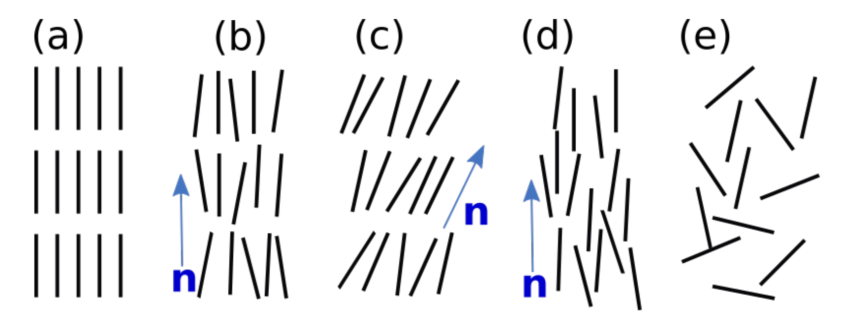
\includegraphics[width=0.95\textwidth]{figures/phases.pdf}
        \end{center}
        \caption{
            Illustrative structures of a substance made up from rod-like molecules.
            In order from (a) to (e) they are a fully crystalized phase, a smectic A, smectic C, nematic and an isotropic liquid.
            $\vb{n}$ highlights the nematic orientation.
            Image edited from\cite{pagetComplexTensorsSimple2023}
        }\label{fig:phases}
    \end{figure}
    All, physicists will be well familiar with the ordered crystalline phase, in which the relative positions and possibly orientation of molecules is ordered, predictable and often repeating.
    Liquid crystals (LC) lay between this state and a typical liquid, some aspects of the phase are ordered, but others are not.
    This is best illustrated as a transition from an unordered (isotropic) liquid state as in \cref{fig:phases}.

    In an isotropic liquid the molecules have random, uncorrelated positions and orientations.
    Note that we talk about orientations, these are naturally only present if the molecules themselves are not spherical/symmetric.
    Depending on just how asymmetric they are they can have one or two orientation directions (in 3D), here we mainly look at rod-like molecules which have one, the axis of symmetry.
    The first step in ordering is usually a transition to a nematic liquid crystal in which the orientations of nearby molecules align, see \cref{fig:phases}.
    An important detail of nematic liquid crystals is that the constituent molecules are symmetric along their length as well (the is no head and tail) as this changes the physics, a nematic phase which does not have this symmetry is called a polar nematic.

    Next can come partial positional order, while different classification exist, in essence there are two ways this can happen in 3D.
    Either the translational symmetry is broken along one axis, these are the smectic phases, or along two in the columnar phases\cite{oswaldNematicCholestericLiquid2005}, if the symmetry is broken along three axes we have a fully ordered crystal.
    In the columnar phases there remains only local one direction along which the system is not ordered.
    As such these phases are composed of separated columns of flowing liquid which are at ordered positions much like a 2D crystal.
    In the smectic phases, a broken translational symmetry along one axis results in a layered structure, the system is isotropic and flows within the layers but is organized along the layer normal.
    As such, smectics are fundamentally a layered phase, and that is what we focus on in this project, in essence we develop a mesoscopic model for layering.

    There are various types of smectic phases, the simplest being the smectic A and C shown in \cref{fig:phases}.
    It is worth pointing out that the smectic layering coexists with a nematic order of the molecules.
    In smectic A phases the nematic orientation is always perpendicular to the layering, whereas in smectic C phases these are at an angle.
    Besides these there is a class of hexatic smectic phases, in which the molecules within layers locally arrange in a hexagonal lattice.
    However, while the lattice itself is only maintained for short distances, these local hexatic lattices have an orientation to them as well and this is aligned over large distances.
    Thus these feature yet more order than the smectic A and C phases, they include the B$_\text{hex}$ phase which has the nematic director perpendicular to the layering, along with the F and I phases which have an angle between the two.
    There are also smectic-like crystals which feature fully ordered often hexatic layers, among these are the B and E phases.
    For more details on these structures see \cite{oswaldNematicCholestericLiquid2005,oswaldSmecticColumnarLiquid2005,gennesPhysicsLiquidCrystals1995}.

    \todo[inline,size=\footnotesize]{This could be extended pretty much indefinitely, given the twist data we have perhaps the TGB would be the next thing worth mentioning}
    \todo[inline,size=\footnotesize]{Paragraph on why are they important/useful etc, the usual are soap, displays and hopefully something new? Bacteria! that might need a citation}

    The model presented in this thesis is in its early stages and so we mainly aim to capture the physics of the A and perhaps C phases.
    Though as we have extended the model into 3D it further highlighted that it captures the general concept of layers, and it does not currently have any concept of the underlying nematic order of smectics.
    There is a way to add that and it is perhaps the next step in developing this theory, however it also shows that the model might also be of use in other fields which require a mesoscopic model for layering.
    \todo{I don't like this paragraph but want to mention some of it somehow}

    \subsection{Ginzburg-Landau theory and the nematic \QQ\ tensor}\label{sec:intro_GL_nem}
        Ginzburg-Landau theory is a powerful recipe to build phase transition theories, the work in this thesis being one of them.
        As such we start by introducing these on the example of an isotropic liquid to nematic LC transition for two reasons.
        Because nematic order often underlays smectic order and so the two need to be considered simultaneously, and because the \QQ\ tensor theory for nematics has heavily inspired the \EE\ tensor theory for smectics this thesis is based on.

        \subsubsection{The order parameter}\label{sec:intro_Q}
        The central concept of Ginzburg-Landau theory is the order parameter, this is usually some mathematical object such as a scalar, vector or tensor that has known values for each of the phases and varies in between them in mostly a smooth manner.
        If a single order parameter is used to describe the entire system in question as a whole, it is a Landau theory, one can extract useful information using this alone.
        However, Ginzburg-Landau theory goes a step further and promotes the order parameter to a field.
        This way one may have a part of the system be in one phase and a different part in the other.

        Going back to our example of a nematic LC, this order parameter needs to capture how aligned the molecules are at each point, accounting for the nematic symmetry.
        The way to do this is using the \QQ\ tensor which can be obtained from a system of discrete molecules via
        \begin{equation}
            \du{Q}_\text{mol} = \su{n}_\text{mol}\su{n}_\text{mol} - \frac{\dudelta}{d}
        \end{equation}
        where $\su{n}_\text{mol}$ is a unit vector denoting the orientation of a molecule, $\dudelta$ the identity and $d$ the dimensionality of the system (2 or 3).
        Throughout this thesis we use underlines to denote tensors, the number of underlines being their rank, further if two tensors appear side by side then it means a dyadic/tensor product and any contractions are denoted by dots \nolinebreak $\cdot$ (the contraction order usually does not matter).
        Note that $\du{Q}_\text{mol}$ immediately satisfies the nematic symmetry of to $\su{n}_\text{mol}$ being the same as $-\su{n}_\text{mol}$.
        So each molecule has a $\du{Q}_\text{mol}$ and we take a local average of these to arrive at the tensor field \QQ\ (taking these local minima numerically can be quite tricky).
        Given the form of \QQ\ we can then express it as the following\footnote{This is not quite true in 3D nematics as we discuss later in \cref{sec:intro_Q_biax}.}
        \begin{equation}\label{eq:Qua}
            \du{Q} = S\qty(\su{n} \su{n} - \frac{\dudelta}{d})
        \end{equation}
        where $S$ is a number between 0 and 1, $\su{n}$ is a unit vector and both are fields along with \QQ.
        From there it is easy to see that an isotropic liquid would have $\du{Q} = S = 0$ and a fully nematic one would have $S = 1$ and \nn\ be the orientation of the phase.
        From this it is clear that $\du{Q}$ is a valid order parameter to describe the isotropic to nematic transition, it is in fact the most widely used such parameter due to it respecting the orientational symmetry.

        \subsubsection{The free energy density and deformations}\label{sec:intro_Q_F}
        Now that we have an order parameter, the next step in forming a Ginzburg-Landau theory is to find a suitable free energy, physics then follow through minimization of it.
        This will be a volume integral of a free energy density $f(\su{r})$ over the system and potentially surface contributions $\mathcal{F}(\su{r})$
        \begin{equation}
            F = \int f(\su{r}) dV + \int \mathcal{F}(\su{r}) dS
        \end{equation}
        though the surface is often dealt with separately.
        $f(\su{r})$ should only depend on the order parameter \QQ\ and elastic constants, it must be local, and crucially it must maintain any symmetries of the system\cite{kardarStatisticalPhysicsFields2007,reichlModernCourseStatistical2016}.
        This can be done in two ways, if one know the underlying microscopic interactions then these can be coarse-grained to obtain $f(\su{r})$.
        However, this can be very difficult or not possible at all, and one might not know all the microscopic interactions.
        This is where the power of Ginzburg-Landau theories lays as one may instead start taking all possible symmetry-allowed terms of $f(\su{r})$ increasing in power of the order parameter and stop once all the physics is captured\todo{could use a citation, got this from StatPhys notes}.
        % This approach will only be valid near the critical point and under 

        In the example of \QQ, that already contains the $\su{n} \leftrightarrow -\su{n}$ symmetry and the bulk free energy density (which does not account for gradients) should only depend on $S$ as it should be the same regardless of the orientation direction.
        As such we have $f_\text{bulk}(\su{r})$ being a power series of $S$ and given \cref{eq:Qua} that translates to a series of suitably contracted terms of \QQ.
        Generally, the following form is used
        \begin{equation}\label{eq:Qfbulk}
            f_\text{bulk}(\su{r}) = \frac{a}{2} \Tr(\du{Q}^2) - \frac{b}{3} \Tr(\du{Q}^3) + \frac{c}{4} \Tr(\du{Q}^2)^2 = \frac{a}{2} Q_{ij}Q_{ij} - \frac{b}{3} Q_{ij}Q_{jk}Q_{ki} + \frac{c}{4} Q_{ij}Q_{ij}Q_{kl}Q_{kl}
        \end{equation}
        where $b$ and $c$ are positive constants and $a$ can have either sign, the terms correspond to $S^2, S^3$ and $S^4$ terms\cite{brayTheoryPhaseOrdering1993,luckhurstBiaxialNematicLiquid2015}.
        The repeated indices in the second form of \cref{eq:Qfbulk} being Einstein summation indices which are assumed throughout this thesis unless otherwise specified.
        This form can have one or two minima for $S\geq0$, this is determined by the coefficients which are set relative to a critical temperature or concentration.
        Without going through the details, generally one takes enough terms to allow for a suitable number of minima (each of which corresponds to a stable or metastable phase), then one extra term with a positive coefficient is added to make sure that $f_\text{bulk}(\su{r})$ keeps growing at very large order parameter.

        However, $f_\text{bulk}(\su{r})$ does not account for any deformation energy costs, which is naturally a key ingredient to describing a system.
        To add these we introduce terms to $f(\su{r})$ which depend on the gradients of the order parameter.
        This gets more complex, though the same rule still applies, take as many allowed terms in increasing powers of the order parameter and \mgrad\ as is needed.
        However, here finding the correct form can get tricky and one generally starts considering specific geometries of the system and what their deformation terms should be like.
        If one is to work analytically or on a constrained system, it might also be that certain terms are negligible and others are not, as such, which terms are used varies in literature.

        \begin{figure}[t]
            \begin{center}
                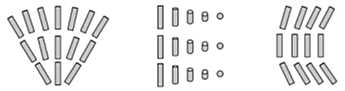
\includegraphics[width=0.6\textwidth]{figures/nematic_deformations.jpg}
            \end{center}
            \caption{
                Diagrams of the splay, twist and bend nematic deformation types respectively.
                Image taken from \cite{suryantariImageFeatureExtraction2019}.
            }\label{fig:nem_deform}
        \end{figure}

        For the nematic case, in the simplest case of constant $S$ but varying \nn\ we get the Frank-Oseen deformation energy terms\cite{brayTheoryPhaseOrdering1993,frankLiquidCrystalsTheory1958,gennesPhysicsLiquidCrystals1995}
        \begin{align}
            K_1 (\mgrad \cdot \su{n})^2 && K_2 (\su{n} \cdot \mgrad \times \su{n})^2 && K_3 (\su{n} \times \mgrad \times \su{n})^2
        \end{align}
        where the $K_?$\todo{is this okay?} are positive elastic constants.
        These three terms correspond to three type of deformation of the director \nn: splay, twist and bend respectively, as shown in \cref{fig:nem_deform}.
        Adapting these to be in terms of \QQ\ has proven difficult, first attempted by de Gennes\cite{gennesPhysicsLiquidCrystals1995} using the terms
        \begin{align}
            L_1Q_{ij,k}Q_{ij,k} && L_2Q_{ij,j}Q_{ik,k} && L_4\epsilon_{ijk}Q_{il}Q_{jl,k}
        \end{align}
        with $L$s being elastic constants and $\epsilon$ the Levi-Civita tensor.
        However, these have later been shown to imply $K_1 = K_3$\cite{lubenskyMolecularDescriptionNematic1970}, which is contradicted by experiment.
        Since then additional terms have been added to account for this\cite{longaExtensionLandauGinzburgdeGennes1987} though that is going beyond the scope of this summary.
        What is worth noting however is the one constant approximation, where all the $K$ elastic constants are taken to be equal which leads to all the terms collapsing to
        \begin{equation}
            L_1 Q_{ij,k}Q_{ij,k}
        \end{equation}
        While this is the simplest possible approximation, it has been used widely for both numerical and analytical studies, and historically it has been the starting point before the different terms have all been discovered.\todo{Not sure the second part is true...}
        In many ways it highlights the idea of Ginzburg-Landau theory in that it is the simplest possible term one can construct using \QQ\ and \mgrad\ and it captures all the possible deformation terms.
        In the work on smectics presented in this thesis we start from a similar approximation, still using it but also trying to go a step beyond and develop more specific terms which collapse to the approximation.


        \subsubsection{Biaxial nematics and \QQ}\label{sec:intro_Q_biax}
        There is one additional bit of complexity worth introducing and that is biaxiality of nematics.
        We have been talking about the orientation of molecules as being a single direction, which is correct for rod-like molecules.
        However, if the molecules are completely asymmetric then there can be order in two perpendicular directions.
        Say we have long cuboid molecules, they can first order by aligning their longest axes and then also rotate around those axes so that the next longest axes also align.
        The same applies to any asymmetrical shaped molecules in 3D (this cannot happen in 2D as there are less orientational degrees of freedom).

        It demonstrates the power of \QQ\ that we can still use it to describe this dual order, we can still calculate it exactly the same way through $\du{Q}_\text{mol}$ and \QQ\ will still be symmetric and traceless, however we now allow it to take the more general form
        \begin{equation}\label{eq:Qbiax}
            \du{Q} = S_1\qty(\su{n} \su{n} - \frac{\dudelta}{d}) + S_2\qty(\su{m} \su{m} - \frac{\dudelta}{d})
        \end{equation}
        where $\su{n}$ and $\su{m}$ are mutually orthogonal unit vectors which describe the directions of the two orders, with $S_1$ and $S_2$ acting as their corresponding order parameters.

        This more general type of nematic order comes with many complications especially when it comes to the free energy forms as it is difficult to separate the two orders contained in \QQ.
        However, it has been extensively studied during the last decades with fascinating phases being used including those of banana shaped molecules\cite{luckhurstBiaxialNematicLiquid2015,kumarBiaxialityNematicSmectic2017,kimCurvaturesSmecticLiquid2018}.

    \subsection{Describing smectics\cite{oswaldSmecticColumnarLiquid2005}}\label{sec:intro_degen}
        Fundamentally, the layered positional order corresponds to a wave-like density fluctuation.
        Following \cite{oswaldSmecticColumnarLiquid2005} in the approach suggested by de Gennes, if we first only consider a single wave throughout the entire system, then the density field is
        \begin{equation}\label{eq:density_base}
            \rho(\su{r}) = \rho_0 + \rho_1\cos(\su{q_0}\cdot\su{r} + \phi) = \rho_0 + \Re(\rho_1 e^{i(\ssu{q_0} \cdot \ssu{r} + \phi)})
        \end{equation}
        where $\rho_0$ is the average density, $\rho_1$ is the wave amplitude, $\phi$ an arbitrary phase (determined by boundary conditions) and $\su{q_0}$ its wavevector containing both the wave direction ($\su{N} = \frac{\ssu{q_0}}{q_0}$ being the layer normal, the smectic director) and spacing ($\frac{2\pi}{q_0}$).
        This is a very simple start, however already one can take $\rho_1$ as an order parameter (not a field here, making this a Landau theory) with 0 corresponding to no wave and so an isotropic liquid.
        To then build a bulk free energy in terms of $\rho_1$ we need to identify any symmetries.
        The only relevant symmetry here is that of $\rho_1 \leftrightarrow -\rho_1$ as such a change only leads to a change in the phase $\phi$ which is not a physical change.
        Such a change would keep the same wave amplitude and spacing and as such the smectic phase is unchanged and so should be its free energy.
        The implication of this is that the free energy may only have even power terms of $\rho_1$ becoming
        \begin{equation}
            F_\text{bulk} = \frac{A}{2}\rho_1^2 + \frac{B}{4}\rho_1^4 + \frac{C}{6}\rho_1^6 + \cdots
        \end{equation}
        with $A, B, C$ being constants which determine the order of the isotropic-smectic phase transition\cite{oswaldSmecticColumnarLiquid2005}.

        The natural next step is to promote $\rho_1$ to a field and the free energy to a free energy density, this leads to equivalent bulk terms but also deformation terms.
        In that case the layering direction and spacing is uniform throughout the system, however the ordering can be perfectly smectic or perfectly isotropic in different areas.
        To account for local changes to layering direction and spacing one must allow some part of the phase of \cref{eq:density_base} to change in space.

        Different choices can be made in that regard, the first and most commonly used being to keep $\su{q_0}$ constant but make $\phi$ a field.
        This allows the layers to locally contract, dilate and tilt in small magnitudes as the phase changes through $\phi$.
        This is a particularly good approach to study near equilibrium configurations, their stability and energetics as it contains enough information yet is simple enough for analytical work.
        Going a step  further, $\su{q_0}$ need not be constant throughout the system as long as we keep it fixed in time.
        This way more interesting geometries can be studied through an imposed $\su{q_0}$ and solving for $\rho_1$ and $\phi$.

        It is worth elaborating a little on what exactly $\phi$ means once we have made it a field.
        It is difficult to quantify how exactly it may alter the layering direction and so we do not discuss that here, however there is a clear correspondence between gradients in $\phi$ and contractions and dilations.
        For simplicty, consider a 1D system with $\phi = s x$ where $s$ is a constant gradient, then clearly we have $e^{i(q_0 x + s x)} = e^{i(q_0 + s) x}$ or in other words we simply have a modified wavelength of $\frac{2\pi}{q_0 + s}$.
        For a more complex example see \cref{fig:gradphi} where we have a spherically symmetric setup of $\su{q_0} = \frac{2\pi}{2\si{L}} \hat{\su{r}}$ with \si{L} being an arbitrary unit of length and
        \begin{equation}\label{eq:gradphi_phi}
            \phi(\su{r}) = \begin{cases} 0 & \qq{if} r \leq 5\si{L} \\ s(r - 5\si{L}) & \qq{if} r \geq 5\si{L} \end{cases}
        \end{equation}
        In other words, $\phi$ has a constant gradient of $s$ in the layering normal direction for $r\geq5\si{L}$ which results in a constant change to layer spacing.
        The key point here being that gradients of $\phi$ in the direction of layering correspond to contractions and dilations.

        \begin{figure}[t]
            \begin{center}
                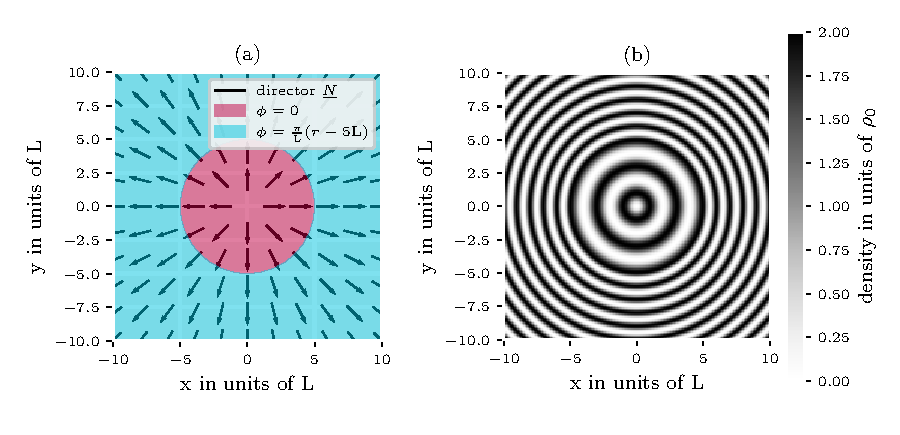
\includegraphics{figures/misc/wave_phi_example.pdf}
            \end{center}
            \caption{
                Diagrams of how \cref{eq:density_base} behaves for a 2D, spherically symmetric system with a non-uniform but fixed $\su{q_0} = \frac{2\pi}{2\si{L}}\hat{\su{r}}$, constant $\rho_1 = \rho_0$ (so a fully smectic phase) and $\phi$ given by \cref{eq:gradphi_phi} with $s=\frac{\pi}{\si{L}}$.
                \si{L} here is an arbitrary unit of length.
                (a) shows the layer normal direction \NN\ and highlights the two zones for $\phi$.
                (b) shows the resulting density having constant wavelengths of $2\si{L}$ and $\frac{2\pi}{\frac{2\pi}{2\si{L}}+\frac{\pi}{\si{L}}} = 1\si{L}$ in each of the zones from (a).
            }\label{fig:gradphi}
        \end{figure}

        In these approaches a complex order parameter $\psi=\rho_1e^{i\phi}$ is used to simplify \cref{eq:density_base} to $\rho(\su{r}) = \rho_0 + \Re(\psi(\su{r}) e^{i\ssu{q_0}\cdot\ssu{r}})$, this is known as the de Gennes order parameter.
        In essence, it replaces the degrees of freedom of two real parameters by a single complex one.
        It is using this theory that de Gennes has demonstrated an analogy between smectic liquid crystals and superconductors\cite{degennesAnalogySuperconductorsSmectics1972}, a particularly fruitful contribution leading to better understanding of the twist-grain boundary phase\cite{lubenskyTwistgrainboundaryPhasesNematic1990} among others.

    \subsection{Smectic (and nematic) defects}
    There is one more prevalent topic of liquid crystals worth introducing before we start discussing issues of the de Gennes complex order parameter and that is defects.
    In general those are some type of localized irregularities in the structure of a liquid crystalline phase.
    For smectics there two main types, disclinations which are defects of the director \NN\ field and dislocations which are additional layers which are not matched and abruptly end.
    In this section we provide a brief introduction to disclination defects, which are common to both smectics and nematics, as the model we work on for smectics is a mesoscopic one and we do not expect it to be able to resolve dislocations.

    Disclinations are points, lines or planes where some underlying orientation field is discontinuous.
    Simplest examples are the 2D point defects shown in \cref{fig:defects} for a vector-like field.
    We say vector like as this field may be more symmetric than a vector, like say the orientation of our rod-like molecules.

    An important concept that comes with disclination defects is topoligical charge.
    In 2D one can calculate the topological charge of a point disclination by encircling it counterclockwise with a closed contour and summing the total orientational change that takes place along it.
    This is then divided by $2\pi$ to obtain the topological charge, perhaps the simplest disclination to try this on is the vortex seen in \cref{fig:defects}(b).
    Topological charge is important because the symmetries of the underlying field determine what charge disclinations a system can have.
    This is as the point defects are precisely that, points, we must have the orientation continuous everywhere else and so for a $+\frac{1}{2}$ disclination to not result in a discontinuety somewhere around it we much have parity symmetry of the underlying vector field.

    Given this in nematic and smectic liquid crystals we mainly consider half integer defects due to their respective symmetries.
    However, other approaches and ideas exist, in fact recently Monderkamp et al\cite{monderkampTopologyOrientationalDefects2021,a.monderkampTopologicalFineStructure2022} have suggested a tetratic symmetry for smectics as they have observed point-like $\pm\frac{1}{4}$ charge defects and lines corresponding to half integer defects.
    It is worth noting that generalizing topological charges to 3D is not as straight forward as one might hope, but we do not discuss that here as we will not be needing it.

    \begin{figure}[t]
        \begin{center}
            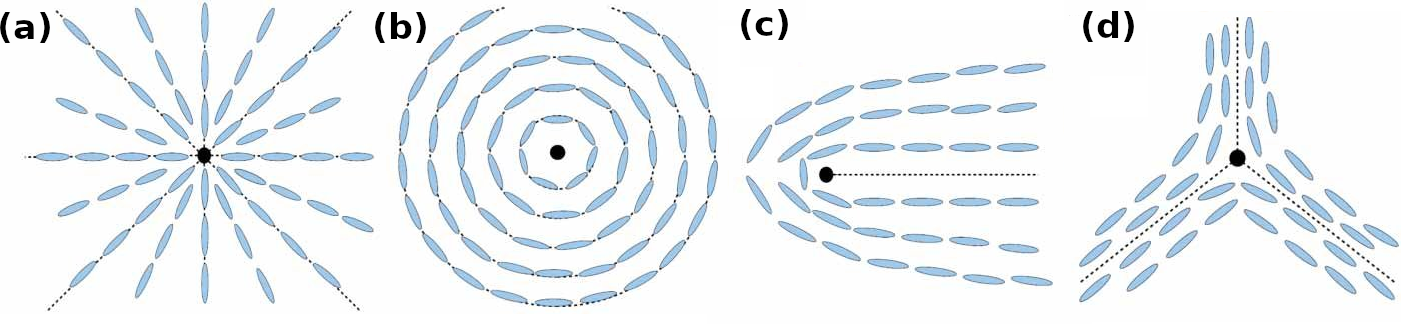
\includegraphics[width=0.95\textwidth]{figures/nematic_defects.png}
        \end{center}
        \caption{
            Diagrams of the simplest point disclinations in 2D.
            The blue ovals depict the orientation field with the black dots being the disclination points where the orientation is discontinuous.
            (a-b) are the aster and vortex (both topological charge +1), and (c-d) are the comet (charge $+\frac{1}{2}$) and triradius (charge $-\frac{1}{2}$). Figure edited from \cite{foffanoDynamicsColloidalIntrusions2014}.
        }\label{fig:defects}
    \end{figure}

    \subsection{Limitations of $\psi$ and the $\su{N} \leftrightarrow -\su{N}$ symmetry}\label{sec:intro_pevnyi}
        The theoretical framework described in \cref{sec:intro_degen} has been very successfully used since the second half of the 20th to understand many of the smectic and other liquid crystalline phases\todo{needs citations...}.
        However, it also comes with some significant shortcomings, two of which have been highlighted by Pevnyi, Selinger and Sluckin in 2014\cite{pevnyiModelingSmecticLayers2014} and which have sparked renewed interest in smectic studies.
        As a response a new smectic order parameter \EE\ has been developed along with a corresponding free energy form by Paget et al\cite{pagetComplexTensorsSimple2023,pagetSmecticLayeringLandau2022,pagetComplextensorTheorySimple2023} and this thesis continues that work.

        The main issue arises when studying the dynamics of more complex systems as when studying a how different domains may form during the isotropic to smectic transition and how they then merge and defects annihilate\cite{ambrozicAnnihilationEdgeDislocations2004,abukhdeirDefectKineticsDynamics2008}.
        In these cases the mentioned approach of keeping $\su{q_0}$ fixed and only working with $\rho_1$ and $\phi$ from \cref{eq:density_base} cannot work.
        In theoretical studies this can often be circumvented by separating the system into domains manually, however this is not feasible for numerical studies.
        If one is to model such a complex system using a single set of fields, a slightly different complex order parameter is used which replaces all the degrees of freedom from \cref{eq:density_base}\cite{mukherjeeSimpleLandauModel2001,mukherjeeAdvancesIsotropicSmectic2021}.
        Mathematically this is equivalent to setting $\su{q_0} = 0$ with us now having
        \begin{equation}\label{eq:density_pevnyi}
            \rho(\su{r}) = \rho_0 + \Re(\psi(\su{r}))
        \end{equation}
        and $\phi$ carrying all of the phase information including the layering direction and spacing.
        The layering wavevector can then be recovered via $\su{q_0} = \mgrad \phi$ and so the layering normal direction is $\su{N} = \frac{\mgrad \phi}{|\mgrad \phi|}$.

        \begin{figure}[t]
            \begin{center}
                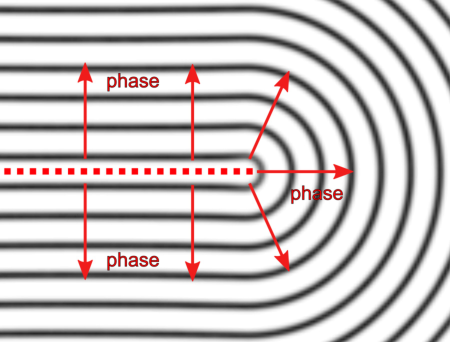
\includegraphics[width=0.4\textwidth]{figures/pevnyi.pdf}
            \end{center}
            \caption{
                Diagram of a $+\frac{1}{2}$ defect in the smectic phase to demonstrate the double-valuedness of the de Gennes complex order parameter, taken from \cite{pevnyiModelingSmecticLayers2014}.
                Black lines correspond to smectic layers, red arrows point in the direction of increasing (or decreasing, this is a choice) $\phi$.
                Dotted red line is where the gradient of $\phi$ discontinuously changes (this can be chosen to be elsewhere) even though the layering there is uniform.
            }\label{fig:pevnyi}
        \end{figure}

        This is the order parameter that Pevnyi et al discuss and the main problem they bring up is that $\psi$ is fundamentally double-valued, or in other words ill-defined.
        Why this is perhaps best shown on the example of a smectic system with a $+\frac{1}{2}$ defect, as in \cref{fig:pevnyi}.
        In order to obtain such layering in the model of \cref{eq:density_pevnyi} there must be an increasing or decreasing $\phi$ perpendicular to the layering.
        Now consider it is increasing downwards in the bottom half of \cref{fig:pevnyi}, then as $\phi$ ought to be smooth in the defect free region to its right and around the defect, we end up with an upwards increasing $\phi$ in the upper region of \cref{fig:pevnyi}.
        This then gives a line of a discontinuous change in $\su{N} = \mgrad \phi$ in the middle left, along the highlighted line, which is also defect free and so any fields should be changing smoothly.

        Ultimately this double-valuedness is a result of the smectic $\su{N} \leftrightarrow -\su{N}$ symmetry as layering upwards and downwards is physically the same.
        This is exactly what we see in the left part of \cref{fig:pevnyi} where we get \NN\ pointing downwards in the bottom half and upwards in the upper half.
        The problematic middle line is unclear, however in a physical sense both directors are equivalent and the phase is continuous.
        This problem is not a purely formal one either, unless accounted for it leads to unphysical line defects appearing between point defects\cite{pevnyiModelingSmecticLayers2014} and associated unphysical energy costs.
        This is the key problem that \EE\ theory aims to solve.

    \subsection{Other recent approaches to simulating smectics}\label{sec:intro_sm_other}
        Naturally, other approaches to these problems have been developed as well.
        Pevnyi et al themselves suggest working with the density directly instead of using a coarse-grained mesoscopic order parameter\cite{pevnyiModelingSmecticLayers2014,xiaStructuralLandscapesGeometrically2021,farrellFiniteelementDiscretizationSmectic2023,xiaSimpleTensorialTheory2024}.
        There $\delta\rho(\su{r}) = \rho(\su{r}) - \rho_0 = \Re(\psi(\su{r}))$ is used as the order parameter and a free energy constructed in terms of it.
        In essence this resolves the symmetry problem by switching to a more microscopic picture whereas \NN\ only appears through $\delta\rho$ as a macroscopic variable.
        Of course the free energy must be carefully crafted so that layering does appear, one way to do this is to relate $\delta\rho$ to $\psi$ and use the same free energies that have been developed for $\psi$\cite{pevnyiModelingSmecticLayers2014}.

        Another benefit of this microscopic treatment is that individual layers in the smectic are resolved, unlike in the approaches using $\psi$ where the focus is on the degree of ordering and layer normal direction.
        This is a notable feature as precise layer positioning plays a role in dislocation defects \todo{maybe cref to figure of defect} and it also allows to obtain the preferred layer spacing $q_0$ through simulations instead of considering it as an outside parameter like in most $\psi$ based approaches.
        % The same also applies to $\rho_1$ which can be obtained from simulaltions as opposed to when using $\psi$
        % and the same applies to $\rho_1$ where often $|\psi|$ is taken in the range 0 to 1 (for a fully isotropic and smectic systems respectively) and then scaled by $\rho_1$ (or in fact $\rho_0$) as a physical parameter.

        However, the microscopic nature of this density-based approach is also its largest limitation at it severely limits the size of systems that can be numerically solved for.
        Given that the individual layers need to be captured, in a naive numerical solver many numerical grid points are needed per wavelength $\frac{2\pi}{q_0}$.
        % Given that the individual layers need to be captured, in a naive numerical solver at least on the order of 5 to 10 numerical grid points would be needed per wavelength $\frac{2\pi}{q_0}$.
        In a comparable study using a mesoscopic order parameter only a single grid point might well be sufficient, even less in more uniform areas and perhaps more near defects.

        Additionally, a completely different approach to modelling smectics has also been developed since the end of the last century based on dynamical density functional theory and phase field crystal methods\cite{lowenPhasefieldcrystalModelLiquid2010,elderModelingElasticPlastic2004,achimStabilityLiquidCrystalline2011,vitralPhasefieldModelWeakly2021,nestlerActiveSmecticsSphere2023}.
        This is a rather complex approach which starts at the individual particles, their positions, orientations and interactions and coarse-grains these.
        As such these at a fundamental level describe a more general liquid crystal system of non-spherical (mainly rod-like) particles which may have both nematic and smectic order.
        In the methods of \cite{lowenPhasefieldcrystalModelLiquid2010} one ends up with three fields: the particle density field $\psi_1$, a nematic order parameter $\psi_2$ and the nematic director field $\su{u_0}$.
        The nematic order fields $\psi_2$ and $\su{u_0}$ vaguely corresponding to the $S$ and \nn\ parameters from \cref{sec:intro_Q}.

        This is a promising method, in particular when considering its generality when it comes to different types of order, physical insight and mathematical rigour.
        However, for simulating large mesoscopic systems it shares the same limitations of the density based methods using $\delta\rho$.
        Similarly to those, the smectic ordering is fully captured by a density field (though how that is done is very different) and so it is a microscopic picture of the smectic which limits the scope of numerical simulations.

        \todo[inline,size=normalsize]{Maybe add something about Monderkampf simulation results?}

\section{Introduction to \EE\ Theory}\label{sec:Ei}
    In this chapter we introduce \EE\ theory, a Ginzburg-Landau theory for smectic liquid crystals and perhaps other layered systems as developed by Paget, Shendruk et al\cite{pagetComplexTensorsSimple2023,pagetSmecticLayeringLandau2022,pagetComplextensorTheorySimple2023} and continued as a part of this thesis.
    Firstly, to revise the main objectives and motivations for \EE.
    The goal is to develop a mesoscopic order parameter of layering that is suitable for large numerical simulations.
    Mesoscopic meaning that it does not resolve individual layers but only their overall ordering, direction and spacing.
    To start, the focus is in particular on the smectic A and perhaps C phases.
    It follows in the approach of de Gennes by using a complex number field, however it must account for the $\su{N} \leftrightarrow -\su{N}$ symmetry in order to avoid unphysical defects.

    As we continue in the spirit of the de Gennes parameter, we start at the density wave equation
    \begin{equation*}
        \rho(\su{r}) = \rho_0 + \Re(\rho_1 e^{i(\ssu{q_0} \cdot \ssu{r} + \phi)}) \tag{\ref{eq:density_base} revisited}
    \end{equation*}
    with the layer normal being $\su{N} = \frac{\ssu{q_0}}{q_0}$.
    We want to build a model capable of describing complex smectic systems, and so we require full flexibility in both the wave amplitude and phase throughout space.
    However, unlike previously when the entire phase of \cref{eq:density_base} was replaced by a phase field $\phi(\su{r})$, here we keep both $\su{q_0}$ and $\phi$ as they are and make them both fields.
    Specifically, we take the magnitude of the wavevector $q_0$ to be a constant physical parameter (perhaps dependent on temperature or other macroscopic variables, though that is not considered here) but allow its direction \NN\ to vary in space.

    So we have three independent fields $\rho_1(\su{r})$, $\su{N}(\su{r})$ and $\phi(\su{r})$, and we would like to form a complex order parameter as before, though to be completely clear it is worth noting the units.
    $\su{N}(\su{r})$ is a dimensionless unit vector, $\phi(\su{r})$ a dimensionless phase but $\rho_1(\su{r})$ has units of density whereas we would like the complex order parameter be dimensionless.
    To achieve that we define $\psi(\su{r}) = \frac{\rho_1(\ssu{r})}{\rho_1}e^{i\phi(\ssu{r})}$ where $\rho_1$ is a constant with units of density that defines the amplitude of the density wave for a fully ordered smectic.
    This leads to
    \begin{equation}\label{eq:rho_ua}
        \rho(\su{r}) = \rho_0 + \rho_1 \Re(\psi(\su{r}) e^{i q_0\ssu{N}(\ssu{r}) \cdot \ssu{r}}) = \rho_0(1 + \frac{\rho_1}{\rho_0} \Re(\psi(\su{r}) e^{i q_0\ssu{N}(\ssu{r}) \cdot \ssu{r}}))
    \end{equation}
    where all the fields are written explicitly, $\psi(\su{r})$ is a dimensionless complex order parameter with magnitude between 0 and 1 and $\rho_0$, $\rho_1$ and $q_0$ are all physical constants defining what a smectic phase would look like on a microscopic level, if one was to make that connection.
    For a further, but reasonable, simplification we may use $\rho_1 = \rho_0$ which is the largest value it may take and it corresponds to a fully smectic phase having the density $\rho(\su{r})$ reach zero in the layer gaps.

    Now we are left with a complex field $\psi(\su{r})$ and a unit vector field $\su{N}(\su{r})$, from now on the explicit field notation will be dropped.
    As established, $|\psi|$ describes how smectic or layered a system is and both \NN\ and $\phi$ influence the phase.
    There is clearly a redundancy between the two, however both are necessary.
    We want a direct way to access \NN\ in order to account for the $\su{N} \leftrightarrow -\su{N}$ symmetry, however using only it would not allow any layer compressions or dilations, and so we must also allow an additional phase $\phi$.
    However, as $\phi$ can also affect the layering direction if it has large gradients in the directions perpendicular to \NN, it is worth noting that the layering direction may be offset from \NN.
    However, in our interpretations we still think of \NN\ as representing the layering direction and gradients of $\phi$ the compressions and dilations (see \cref{fig:gradphi}), this is valid as long as $\phi$ varies slowly compared to \NN\ which is the case in our simulations.

    Now that we have our building blocks ready, we finally need to take account of the $\su{N} \leftrightarrow -\su{N}$ symmetry.
    This is done in analogy to the nematic \QQ\ (\cref{sec:intro_Q}) and we define a new order parameter, the \EE\ tensor, as
    \begin{equation}\label{eq:Eua_def}
        \du{E} = \psi \qty(\su{N}\su{N} - \frac{\du{\delta}}{d})
    \end{equation}
    where $d$ is the number of physical dimensions we consider.
    Just as in the nematic case this immediately enforces the $\su{N} \leftrightarrow -\su{N}$ symmetry and in addition it bundles all of our order parameter fields together.
    This has not been discussed before, but for numerical simulations this comes with another significant advantage as it allows numerical melting in defects.
    To see that consider say an aster-like defect with \NN\ pointing outwards from a point where the phase becomes an isotropic liquid.
    In this system the director \NN\ (and $\phi$ as well) is not well-defined at the point defect and so trying to calculate in numerically leads to issues.
    However, as $|\psi|$ goes to zero at the defect point, so does \EE\ and so it is clearly defined and calculable everywhere.

    As Paget et al note, the tensor field constructed in \cref{eq:Eua_def} is by definition globally gauge invariant (a global shift in phase has no physical effect) and the complex tensor $\du{E}(\su{r})$ at any point is by construction symmetric, traceless and normal.
    A complex tensor is normal if and only if it commutes with its complex conjugate, in other words $[\EE, \EE^*] = 0$ with square brackets denoting the commutator, this follows from \cref{eq:Eua_def} as
    \begin{align}
        [\EE, \EE^*] = \psi\psi^*[\NN\NN - \frac{\dudelta}{d}, \NN\NN - \frac{\dudelta}{d}] = 0
    \end{align}
    and any matrix commutes with itself.
    In a similar fashion, it is useful to consider the contractions of \EE\ as in \cref{eq:Eua_def} with itself, these are
    \begin{align}
        &\EE \cddot \EE = E_{ij}E_{ij} = \psi^2 \frac{d-1}{d} \label{eq:Eua_contr1} \\
        &\EE \cddot \EE^* = |\du{E}|^2 = E_{ij}E_{ij}^* = |\psi|^2 \frac{d-1}{d}\label {eq:Eua_contr2}
    \end{align}
    where we show both the $\cdot$ contraction and Einstein summation notations along with the Frobenius complex matrix norm squared, whenever the form $|\chi|^2$ is used through this thesis it means that one should take $\chi$ and contract over all indices with $\chi^*$ (in order, but it usually does not matter), for scalars this gives the usual $|\psi|^2=\psi\psi^*$.
    From the forms above we can fully recover $|\psi|$ and to some degree also $\phi$ though this requires taking the complex square root and so to choose a branch cut.
    Once we have those, it is easy to use \cref{eq:Eua_def} to reconstruct $\su{N}\su{N}$ and so \NN\ as well.

    \subsection{Free energy in the one constant approximation}\label{sec:Ei_F}
        Now that we have our new order parameter, we need to find a form for the free energy density in terms of it.
        Here we present the simplest possible form that it may take as used by Paget et al\cite{pagetComplexTensorsSimple2023,pagetSmecticLayeringLandau2022,pagetComplextensorTheorySimple2023}.
        This is also heavily inspired by the \QQ\ tensor free energy forms (though we do not make that connection here) with the main difference being that we need to make sure the free energy $F$ is real and not complex.
        Throughout this thesis we only focus on the free energy of the system volume and ignore any surface energies.
        While these are very interesting to study and Paget et al do use them in 2D simulations, we only use fixed or periodic boundary conditions in this thesis and so they do not come into play.

        As in \cref{sec:intro_GL_nem}, we split the free energy density $f(\su{r})$ into a couple of different contributions, the first of which is \FB.
        This is the part that does not depend on deformations and so only depends on constants and \EE, not its gradients.
        It is this term that determines what value does $|\psi|$ take at equilibrium, or in other words whether a system at particular conditions will be in the smectic or liquid phase.
        As before \FB\ will be a series in terms of contractions of \EE, but as we alluded to we must match \EE\ and $\EE^*$ in order to make \FB\ real, the simplest such contraction is $|\du{E}|^2=E_{ij}E_{ij}^*$ ($E_{ii}E_{jj}^*$ cannot be used as \EE\ is traceless) and so we consider \FB\ as a power series given by
        \begin{equation}\label{eq:Efbulk}
            f_\text{bulk} = A |\du{E}|^2 + \frac{C}{2}|\du{E}|^4 = A E_{ij}E_{ij}^* + \frac{C}{2}(E_{ij}E_{ij}^*)^2
        \end{equation}
        where $A$ and $C$ are constants with units of energy per volume as \EE\ is dimensionless, and $C > 0$ to make sure \FB\ has a minimum.
        We only take the first two terms as this is enough to give one minimum in terms of $|\du{E}|^2 = \frac{d-1}{d}|\psi|^2 \geq 0$ at 0 when $A > 0$ for an isotropic liquid or at a non-zero value determined by $A$ and $C$ when $A < 0$ corresponding to the smectic phase.
        More terms could be added in the future to perhaps capture more complex phase transitions but in this work we focus on making sure \EE\ can capture the symmetries and defects of the smectic phase, and so the most important thing is that \EE\ is driven to be non-zero by \FB.

        Moving on to the deformation energy costs, as Paget et al discuss\cite{pagetComplexTensorsSimple2023} smectics have two deformation modes.
        First is that of the mentioned layer compressions and dilations, these are jointly referred to as compressions and we associate a free energy cost \FC\ to them.
        These will depend on gradients on \EE\ and as a first approximation we take these to only depend on the first gradients of \EE.
        The simplest term that can be constructed from $\mgrad \EE$ and is guaranteed to be real is $E_{ij,k}E_{ij,k}^* = |\mgrad \EE|^2$ (any indices after a $,$ denote derivatives, so $\gamma_{,k}=\pdv{x_k}\gamma$) and so in the simplest one constant approximation we use
        \begin{equation}
            \FC = b_1 |\mgrad \EE|^2
        \end{equation}
        with $b_1$ being the compressive elastic constant with units of energy per length.

        The second deformation mode that we wish to consider is the curvature of the layers and as mathematically curvature is captured by second order gradients we expect \FU\ must depend on terms of $\mgrad\mgrad\EE$ (and possibly higher gradients).
        In this thesis we continue from the one constant version of \FU\ suggested by Paget et al which takes the form
        \begin{equation}
            \FU = b_2 |\nabla^2 \EE|^2
        \end{equation}
        with $b_2$ being the curvature elastic constant with units of energy times length.
        Combining these in the double one constant approximation free energy form we have
        \begin{equation}\label{eq:Foca}
            F = \int A |\du{E}|^2 + \frac{C}{2}|\du{E}|^4 + b_1 |\mgrad \EE|^2 + b_2 |\nabla^2 \EE|^2 \dd{V}
        \end{equation}
        which is the simplest reasonable form available and is used and built upon in this thesis.

    \subsection{Order parameter dynamics and functional derivatives}\label{sec:Ei_fdv}
        Now that we have defined the order parameter field \EE\ and found a free energy in terms of it, it is time to discuss the dynamics of \EE.
        There are broadly two types of Ginzburg-Landau theories, those where the order parameter is conserved and those where it is not.
        Say in the density-based smectic theories where the density fluctuation $\delta\rho$ is used as an order parameter (see \cref{sec:intro_sm_other}), there the integral $\int \delta\rho \dd{V}$ must be conserved due to conservation of mass.
        In the case of \EE\ however we have no conservation, almost by definition the system can change from a fully isotropic phase of $\EE=0$ to a fully smectic one with $|\psi|=1 \Leftrightarrow |\EE| = \sqrt{\frac{d-1}{d}}$.

        To start off with a simpler example consider a general system with a non-conserved, real, scalar parameter field $\gamma$.
        For such a system the model A dynamics are well established and given by
        \begin{equation}\label{eq:modA}
            \pdv{\gamma(\su{r})}{t} = -\mu \fdv{F[\gamma]}{\gamma(\su{r})}
        \end{equation}
        where $F[\gamma]$ is the free energy functional, $\fdv{F[\gamma]}{\gamma}$ denotes the functional derivative and $\mu$ is effectively a friction coefficient\cite{kardarStatisticalPhysicsFields2007}.
        We have so far glossed over the functional nature of the free energy $F$, what this means is that the free energy depends "on the whole field" of the order parameter $\gamma$, not just on its value at particular point, integrals such as \cref{eq:Foca} are typically what these look like in physics.
        The functional derivative of the scalar (non-field) $F$ is a field and loosely corresponds to the change in $F$ if we change the value of $\gamma$ at $\su{r}$ by infinitesimal amount, divided by this infinitesimal amount as in normal derivatives.
        Again, in very mathematically loose terms it corresponds to
        \begin{equation}
            \fdv{F[\gamma]}{\gamma(\su{r})} = \lim_{\epsilon \rightarrow 0} \frac{F[\gamma(\su{r'}) + \epsilon\delta(\su{r'} - \su{r})]}{\epsilon}
        \end{equation}
        where $\delta$ is the Dirac delta function and $\su{r'}$ a dummy variable, say the one that is integrated over in the form for $F$.
        In essence the functional nature of $F$ and the use of the functional derivative in \cref{eq:modA} corresponds to having an infinite number of degrees of freedom, one at each point in space, and \cref{eq:modA} tunes each of them separately in order to minimize $F$, while accounting for how they affect each other (through gradient terms in $F$).

        There is, a couple of ways of practically calculating these functional derivatives and a substantial part of this project has been working them out.
        Perhaps the more instructive is to propagate the functional derivative operator $\fdv{\gamma(\ssu{r})}$ into the integral, use the identity $\fdv{\gamma(\ssu{r})}{\gamma(\ssu{r'})} = \delta(\su{r} - \su{r'})$ wherever possible, and when we get terms of the form $\fdv{\gamma(\ssu{r})} \mgrad \gamma$ and similar we integrate by parts.
        This will give an expression for $\fdv{F}{\gamma(\ssu{r})}$ that is a function of $\su{r}$ along with surface integrals coming from the integrations by part.
        These integrals are then ignored for the purposes of \cref{eq:modA} as that is only used for the bulk volume of the system (no surfaces) and the surface terms will contain Dirac deltas that restrict them to only affecting the surface.

        Alternatively and perhaps more commonly a form can be derived for the functional derivative that resembles the Euler-Lagrange equations.
        This form depends on the order of the highest gradient of $\gamma$ present in the form of $F$, say if $F = \int f(\gamma, \mgrad \gamma) \dd{V}$ with $f$ being a free energy density which only depends on the first order gradients of $\gamma$, then we will have
        \begin{equation}
            \fdv{F[\gamma]}{\gamma(\su{r})} = \pdv{f}{\gamma} - \mgrad \cdot \pdv{f}{\mgrad \gamma}
        \end{equation}
        where we only have partial derivatives of $f$ now.
        The second partial derivative is taken with respect to the gradients of $\gamma$ in different directions, which are treated independently to $\gamma$ itself.
        When using this form the surface terms do not explicitly come up, as they are hidden in the derivation of the form, which assumes that we do not vary $\gamma$ or its gradients at the system boundaries.

    \subsection{Dynamics of \EE\ using Wirtinger derivatives}\label{sec:Ei_dyn}
        Now we need to generalize the model A dynamics of \cref{eq:modA} to a complex tensor order parameter.
        Accounting for the tensorial quality is simple, it has been done for \QQ\ before and we take the same approach where each of the components is evolved separately through the same equation.
        For \QQ\ this looks as
        \begin{equation}
            \pdv{Q_{ij}}{t} = -\mu \fdv{F}{Q_{ij}} \quad\Leftrightarrow\quad \pdv{\du{Q}}{t} = -\mu\fdv{F}{\du{Q}}
        \end{equation}
        where $F$ would be a nematic free energy, and we drop both explicit field notation and denoting the functional nature of $F$ with square brackets.

        Accounting for the complex nature of \EE\ is however a little more complicated and it is worth briefly introducing the Wirtinger derivatives\cite{haslingerComplexAnalysisFunctional2017}.
        These are differential operators operating on any real differentiable complex function.
        This means that if we have $f(z) = u(z) + i v(z)$ with $z \in \mathbb{C}$ and $u(z), v(z) \in \mathbb{R}$, then we can use the Wirtinger derivatives as long as $u$ and $v$ are partially differentiable with respect to the real an imaginary parts of $z$.
        This is a much lower bar than a complex function being complex differentiable or even analytical, which is important as neither the complex conjugate $z^*$ nor $z z^* = |z|^2$ are complex differentiable, but they are real differentiable and we have similar terms in our free energy (\cref{eq:Foca}).
        The Wirtinger derivative operators are defined as follows
        \begin{align}
            \pdv{z} &= \frac{1}{2}(\pdv{x} - i\pdv{y}) \\
            \pdv{z^*} &= \frac{1}{2}(\pdv{x} + i\pdv{y})
        \end{align}
        with $x$ and $y$ being the real and imaginary components of $z$ such that $z = x + iy$.
        It is worth noting that for a complex function $f$, if we have $\pdv{f}{z^*}=0$, then $f$ satisfies the Cauchy-Riemann relations which is a necessary condition for complex differentiability.
        Furthermore, if a function $f$ is complex differentiable, then $\pdv{f}{z} = \dv{f}{z}$, in other words its complex derivative if given by its Wirtinger derivative.
        % The important part of these differential operators and why we use them here is the simplicity in using them.
        % When taking a Wirtinger derivative of a complicated function of $z$, insteadd of working with its components $x$ and 

        Where this comes into play is when we consider the optimization of a real function of a complex variable $f(z)$ (similar to our real functional of complex \EE).
        If we want to find a minimum of this function we can solve for $\pdv{f}{x} = \pdv{f}{y} = 0$, where again $z=x+iy$, which is not necessarily a sufficient condition but often works.
        However, if we instead want to iteratively approach a minimum, we can keep stepping in the direction of negative gradient in the complex plane as
        \begin{align}
            x' = x - \epsilon\pdv{f}{x}\label{eq:random1} \\
            y' = y - \epsilon\pdv{f}{y}\label{eq:random2}
        \end{align}
        with $x', y'$ being our next position and $\epsilon$ a parameter.
        This is effectively the same as optimizing a function of a real 2D vector using $\su{u}' = \su{u} - \epsilon \, \mgrad f$, making $\epsilon$ long steps towards a local minimum.
        It is also worth stressing that it is important that $f$ itself is real and not complex as otherwise $x'$ and $y'$ do not stay real, leading to a contradiction.
        In essence this method does not work for complex valued functions as the path from a non-zero complex number to 0 is not unique and one must somehow choose which path to take.

        \Cref{eq:random1,eq:random2} can then be written more efficiently using the Wirtinger derivative as
        \begin{equation}
            z' = z - 2\epsilon \pdv{f}{z^*}
        \end{equation}
        with $z' = x' + y'$.
        Besides just reducing the number of equations we need to track of, the major benefit of using Wirtinger derivatives here is their ease of use.
        When applying these operators to complicated function, we can express that function in terms of $z$ and $z^*$ instead of $x$ and $y$ (using $x = \frac{z+z^*}{2}$ and $y = \frac{z-z^*}{2i}$) and then treat them as if they were independent real variables when taking the Wirtinger derivatives.
        This is best explained by examples, we have $\pdv{z} z = 1, \pdv{z} z^* = 0, \pdv{z} z z^* = z^*$ and similarly for $\pdv{z^*}$, this method holds for more complex mathematical functions like the exponential as well\cite{haslingerComplexAnalysisFunctional2017}.

        Now finally all the ideas are in place to adapt the model A real scalar dynamics of \cref{eq:modA} to a complex tensor order parameter.
        We treat all components independently and use a Wirtinger-like functional derivative to obtain the free energy minimization.
        The final equation is
        \begin{equation}\label{eq:Ei_dyneq}
            \pdv{E_{ij}}{t} = -\mu \fdv{F}{E_{ij}^*} \quad\Leftrightarrow\quad \pdv{\du{E}}{t} = -\mu\fdv{F}{\du{E}^*}
        \end{equation}
        where we evaluate $\fdv{F}{E_{ij}^*}$ by treating each $E_{ij}$ and $E_{ij}^*$ as independent degrees of freedom.
        % Note again that $\mu$ is a friction coefficient and given that \EE\ is dimensionless it has units of inverse time per energy.
        However, the dynamics equation above has a major caveat, it does not in any way account for the form of \EE\ and it does not guarantee that \EE\ will keep the form of \cref{eq:Eua_def}.
        This will be revisited later in \cref{sec:dcE_Edyn2} where we will add Lagrange multiplier terms to it in order to fix that.

\section{New Perspectives on \EE\ in 3D}\label{sec:npE}
    \EE\ theory as presented so far has been based on defining \EE\ in terms of $\psi$ and $\su{N}$ as
    \begin{equation}
        \du{E} = \psi \qty(\su{N}\su{N} - \frac{\du{\delta}}{d}) \tag{\ref{eq:Eua_def} revisited}
    \end{equation}
    however, if we are to treat \EE\ as our order parameter instead of its constituent fields (and only use them for interpretations) we must start treating it as a general complex tensor field, subject to set out constraints.
    This is something that has been rethought as a part of this thesis, in particular when it comes to \EE\ in three dimensions.

    In earlier work\cite{pagetSmecticLayeringLandau2022,pagetComplextensorTheorySimple2023,pagetComplexTensorsSimple2023} \EE\ is identified as symmetric and traceless following the example of \QQ\ and these constraints are clearly necessary for \cref{eq:Eua_def} to hold.
    Symmetry inherently comes from the $\NN\NN$ term that we wish to have.
    And the motivation for adopting a traceless tensor and (so adding the $-\frac{\sdu{\delta}}{d}$ to the necessary $\su{N}\su{N}$) comes down to simplifying the bulk free energy density form (as has been noted in \cref{sec:Ei_F}) which could otherwise have terms of $E_{ii}=\Tr(\du{E})$.
    However, as $\Tr(\su{N}\su{N}) = 1$ due to \NN\ being a unit vector, these terms would only add a constant value to the free energy which may by its nature be subtracted.
    As such making \EE\ (and \QQ) traceless captures the same physics while simplifying the algebra.

    Paget et al cite two more constraints that are put on \EE, the mentioned normality which we show below is in fact a key constraint on \EE, and what is called the uniaxial constraint.
    The term uniaxial is taken in analogy to \QQ\ as in \cref{sec:intro_GL_nem} (in particular \cref{sec:intro_Q_biax}) to mean the exact form of \cref{eq:Eua_def} as opposed to a biaxial form which would look like
    \begin{equation}
        \du{E} = \psi \qty(\su{N}\su{N} - \frac{\du{\delta}}{d}) + \psi' \qty(\su{N'}\su{N'} - \frac{\du{\delta}}{d})
    \end{equation}
    with $\psi'$ and $\su{N}'$ being different complex scalar and unit vector fields.
    The claim is made that the uniaxial form of \cref{eq:Eua_def} will be implied if all components of \EE\ have the same complex phase, in order words if we can write
    \begin{equation}
        \EE = e^{i\alpha} \du{R}
    \end{equation}
    with $\alpha$ a real number $\du{R}$ a real matrix.
    Further, this is stated that this is satisfied if $\det([\EE,\EE^*]) = 0$ via an argument parametrizing \EE\ through angles which we do not repeat here.
    In contradiction to that, we claim here that the uniaxial form of \cref{eq:Eua_def} is not guaranteed even if all components of \EE\ have the same complex phase and question whether requiring $\det([\EE,\EE^*])=0$ has any effect once we have already required the stronger constraint of normality, $[\EE,\EE^*]=0$.
    However, it should be noted that Paget et al only worked in two dimensions where as they correctly state the constraints $[\EE,\EE^*]=0$ and $\det([\EE,\EE^*])=0$ are fully equivalent (\cref{app:noruaeq}), and they practically only enforce the so called uniaxiality constraint which enforces normality, and as we shall show, in 2D that is enough to guarantee uniaxiality.

    \subsection{Requiring \EE\ to be symmetric, traceless and normal}\label{sec:npE_cnst}
        It is now time to determine what form can we restrict \EE\ to, using which constraints and how.
        We will work in three dimensions in the derivation below though it generalizes and we hope the make any points that change clear.
        We expect symmetry and tracelessness to be upheld and with the benefit of hindsight claim normality to be the key additional constraint.
        This is as besides the statement $[\EE,\EE^*]=0$ which has the convenient form of a holonomic constraint, normality of a complex matrix is also equivalent to it being diagonalizable by a unitary matrix.
        Thus, in 3D we can write a normal \EE\ as
        \begin{align}
            \du{E} &= \du{U} \cdot \begin{pmatrix}
                \lambda_1 & 0 & 0 \\
                0 & \lambda_2 & 0 \\
                0 & 0 & \lambda_3 \\
            \end{pmatrix} \cdot \du{U}^\dagger \label{eq:Ederstart} \\
            \intertext{
            where $\du{U}$ is a unitary matrix (so $\du{U}^{-1} = \du{U}^\dagger$) the columns of which are the eigenvectors of \EE\ and $\lambda_1,\lambda_2$ and $\lambda_3$ are their corresponding eigenvalues.
            Firstly, we can remove one degree of freedom from the inner matrix by using the identity matrix with
            }
            % \du{E} &= \du{U} \cdot \qty(\begin{pmatrix}
            %     \lambda_1 - \lambda_3 & 0 & 0 \\
            %     0 & \lambda_1 - \lambda_3 & 0 \\
            %     0 & 0 & 0
            % \end{pmatrix} +\lambda_3\du{\delta}) \cdot \du{U}^\dagger \\
            \du{E} &= \du{U} \cdot \begin{pmatrix}
                \lambda_1 - \lambda_3 & 0 & 0 \\
                0 & \lambda_2 - \lambda_3 & 0 \\
                0 & 0 & 0
            \end{pmatrix} \cdot \du{U}^\dagger + \lambda_3\dudelta
        \end{align}
        as $\du{U} \cdot \dudelta \cdot \du{U}^\dagger = \dudelta$.

        Now, when doing the matrix multiplication each of the diagonal components will only interact with one of the eigenvectors in $\du{U}$, in index notation we have
        \begin{equation}\label{eq:Edermid}
            E_{ij} = U_{i1}(\lambda_1 - \lambda_3)U_{1j}^\dagger + U_{i2}(\lambda_2 - \lambda_3)U_{2j}^\dagger + \lambda_3 \delta_{ij}
        \end{equation}
        and using the definition of the hermitian conjugate and denoting the eigenvectors of \EE\ and columns of $\du{U}$ as $\su{U_k}$ this gives
        \begin{align}
            \du{E} &= (\lambda_1 - \lambda_3) \su{U_1}\su{U_1^*} + (\lambda_2 - \lambda_3) \su{U_2}\su{U_2^*} + \lambda_3 \du{\delta} \\
            \intertext{
            which starts featuring dyadic products of vectors, as does \EE.
            If we now impose tracelessness through requiring that $\lambda_3 = -\lambda_1-\lambda_2$ (trace is invariant to unitary transformations and so $\Tr(\du{E})$ is given by the sum of its eigenvalues) we arrive at
            }
            \du{E} &= (\lambda_1 - \lambda_3) \su{U_1}\su{U_1^*} + (\lambda_2 - \lambda_3) \su{U_2}\su{U_2^*} + \frac{-(\lambda_1 - \lambda_3)-(\lambda_2 - \lambda_3)}{3} \du{\delta} \\
            \du{E} &= \psi_1 \qty(\su{U_1}\su{U_1^*} - \frac{\dudelta}{3}) + \psi_2 \qty(\su{U_2}\su{U_2^*} - \frac{\dudelta}{3})\label{eq:Edernearlythere}
        \end{align}
        with $\psi_i = \lambda_i - \lambda_3$ for $i < d$ and which now nearly matches the biaxial form for \EE, though with complex vectors present.

        For the final step, recall that the columns (and rows) of a unitary matrix are normalized and mutually orthogonal, this means we can parametrize any of the columns as
        \begin{equation}
            \su{U_k} = \begin{pmatrix} R_1 e^{i\phi_1} \\ R_2 e^{i\phi_2} \\ R_3 e^{i\phi_3} \end{pmatrix}
        \end{equation}
        with $R_1, R_2, R_3 \geq 0$, $R_1^2+R_2^2+R_3^2 = 1$ and $\phi_1,\phi_2,\phi_3$ being complex phases (no relation to $\phi$ from before).
        Then we impose symmetry on \EE\ through requiring $\EE=\EE^\text{T}$ on \cref{eq:Edermid} which leads to
        \begin{equation}
            \su{U_k}\su{U_k^*} = \su{U_k^*}\su{U_k} \qq{no Einstein summation over $k$}
        \end{equation}
        holding for each $k < d$.
        Solving this matrix equation in terms of the parametrization gives no further restriction on the $R_i$ but we get that for any $i, j$
        \begin{equation}
            e^{i(\phi_i - \phi_j)} = e^{i(\phi_j - \phi_i)}
        \end{equation}
        or in other words the phases of the components of $\su{U_k}$ must differ by a multiple of $\pi$.
        While this does not necessarily imply $\su{U_k}$ must be real (after all eigenvectors are only unique up to multiplication which can include complex phases) it does have implications for the dyadic products appearing in \cref{eq:Edernearlythere} which take the form
        \begin{equation}
            \su{U_k}\su{U_k^*} \leftrightarrow \begin{pmatrix}
                R_1^2 & R_1 R_2 e^{i(\phi_1-\phi_2)} & R_1 R_3 e^{i(\phi_1-\phi_3)} \\
                R_1 R_2 e^{-i(\phi_1-\phi_2)} & R_2^2 & R_2 R_3 e^{i(\phi_2-\phi_3)} \\
                R_1 R_3 e^{-i(\phi_1-\phi_3)} & R_2 R_3 e^{-i(\phi_2-\phi_3)} & R_3^2
            \end{pmatrix}
        \end{equation}
        and so the dyadic products are fully real with the signs of the components being determined by whether their corresponding phase difference is an odd or even multiple of $\pi$.
        Thus, any such term can be replaced by the dyadic product of a real vector with itself which may even be restricted to the upper half space ($z \geq 0$) highlighting the inherent symmetry of \EE\ with respect to its inbuilt directionality.

        Coming back to \EE\ in 3D and following up from \cref{eq:Edernearlythere}, the argument above applies to both $\su{U_1}$ and $\su{U_2}$ along with the unitarity of $\du{U}$ also making sure they are mutually orthogonal.
        As such we may replace them in notation by real, mutually orthogonal unit eigenvectors of \EE, \NN\ and \MM\ which each correspond to one eigenvalue.
        This gives exactly the biaxial form of
        \begin{equation}\label{eq:Ebiax}
            \du{E} = \psi_1 \qty(\NN\NN - \frac{\dudelta}{3}) + \psi_2 \qty(\MM\MM - \frac{\dudelta}{3})
        \end{equation}
        which is a general form that any symmetric, traceless and normal complex matrix can be put in.
        This accounts for all the degrees of freedom with \NN\ and \MM\ capturing those of two its eigenvectors (the third is fully determined through their mutual orthogonality and symmetry of \EE) and the $\psi_i$ capturing those of their corresponding eigenvalues (the third being determined by tracelessness of \EE).
        Recall that we have $\psi_i = \lambda_i - \lambda_3$, so we have an invertible transformation
        \begin{equation}
            \begin{pmatrix} \psi_1 \\ \psi_2 \end{pmatrix} = \begin{pmatrix} 2 & 1 \\ 1 & 2 \end{pmatrix} \begin{pmatrix} \lambda_1 \\ \lambda_2 \end{pmatrix}
            \quad\Leftrightarrow\quad
            \begin{pmatrix} \lambda_1 \\ \lambda_2 \end{pmatrix} = \frac{1}{3}\begin{pmatrix} 2 & -1 \\ -1 & 2 \end{pmatrix} \begin{pmatrix} \psi_1 \\ \psi_2 \end{pmatrix}
        \end{equation}

        Finally, it is worth pointing out exactly how this generalizes to different dimensionalities.
        For a $d$ dimensional system a general \EE\ would have $d$ eigenvalues along the diagonal in \cref{eq:Ederstart}, one of which we are able to remove from the matrix product and form the $\dudelta$ term.
        So we would then arrive at $d-1$ terms involving eigenvalue differences and dyadic products of eigenvectors.
        The only other difference is that the number $3$ present in the denominator once we use the tracelessness property would become a general $d$, so in a $d$ dimensional system \EE\ would take the form of
        \begin{equation}\label{eq:Emultiax}
            \du{E} = \psi_1 \qty(\su{N_1}\su{N_1} - \frac{\dudelta}{d}) + \psi_2 \qty(\su{N_2}\su{N_2} - \frac{\dudelta}{d}) + \cdots + \psi_{d-1} \qty(\su{N_{d-1}}\su{N_{d-1}} - \frac{\dudelta}{d})
        \end{equation}
        which may be called a multiaxial form to be general, though we do not see a reason to consider systems with $d>3$.

    \subsection{Interpreting biaxiality in 3D}
        First thing to note about the results from the previous section is that as was mentioned, in 2D we do not need any further constraints on \EE\ besides symmetry, tracelessness and normality to guarantee a uniaxial \EE.
        This clearly follows from \cref{eq:Emultiax}.
        However in 3D things get more difficult, firstly to address the suggested constraint of all components of \EE\ having the same complex phase.
        It is worth noting that this really means up to a factor of $\pi$ as we clearly want to allow components to differ by a sign.
        Even if we have an \EE\ of form \cref{eq:Ebiax} with $\psi_1$ and $\psi_2$ having the same phase and so satisfying the constraint, given that \NN\ and \MM\ are mutually orthogonal there is no way to combine the two terms into one.
        As such, we drop the single complex phase constraint and examine whether it is possible to constrain \EE\ to be uniaxial.

        One way to approach this problem is to notice that the biaxial form of \cref{eq:Ebiax} becomes the uniaxial form if one of the $\psi_i$ is 0.
        This leads to the problem of constraining uniaxiality, as recall that the $\psi_i$ are differences of their corresponding eigenvalues $\lambda_i$ and the one we chose to take out during the derivation, say $\lambda_3$.
        As such requiring a $\psi_i$ to be 0 is the same as requiring some two eigenvalues to be equal.
        This is a very problematic type of constraint as it fundamentally requires us to directly constrain the eigenvalues of the matrix which are not analytically accessible.
        What is meant by this is that there is no usable analytic form for the eigenvalues of a general matrix, that they do not come in a clear order and can be degenerate.
        These features make constraining \EE\ to have two equal eigenvalues unworkable for us, especially as we will be using Lagrange multipliers to enforce the constraints and for that to be possible they must take the form a holonomic constraint $f(\du{E}) = 0$.

        As such, we in this thesis allow \EE\ to be biaxial in 3D.
        Initially this decision was also guided by the example of \QQ\ which in 3D also gains a biaxial term that is difficult to remove (see \cref{sec:intro_Q_biax}).
        However, in simulations of \QQ, in the final, static states the biaxiality is only present in or near defects.
        We expected \EE\ to behave in the same way and for the final states of our simulations to have regions of uniaxial \EE\ with biaxiality only near defects and largely negligible, however this did not turn out to be the case.

        Given that, we attempt to interpret the biaxiality of \EE.
        Firstly, recall that the biaxiality of \QQ\ in nematics corresponds to asymmetric constituent molecules and so us having two directions of orientational order.
        Thus the biaxiality of \QQ\ corresponds to the biaxiality of the molecules.
        In \cref{sec:intro} we have explained how a typical smectic phase forms through layers developing in a uniaxial nematic phase.
        There is also a class of layered biaxial nematic phases, where both orientational directions of asymmetric molecules are aligned and there is also layering.
        These are called biaxial smectics\cite{k.sadashivaBiaxialSmecticPhase2002,semmlerBiaxialSmecticPhases1998} and it is very important to stress that we do not believe these to be in any way related to the biaxiality of \EE\ that we see here.
        The biaxiality in biaxial smectics corresponds to the nematic biaxiality and smectic layering is defined positional symmetry breaking only in one direction.

        However, we are getting a biaxial \EE\ and we suggest that just as an additional term in \QQ\ corresponds to an additional orientational order, any additional terms in \EE\ correspond to additional layering order.
        Recall that we interpret the uniaxial form of $\EE = \psi (\NN\NN - \frac{\sdu{\delta}}{d})$ as density wave in the direction of \NN\ given by \cref{eq:rho_ua}.
        As such we interpret
        \begin{equation}
            \du{E} = \psi_1 \qty(\NN\NN - \frac{\dudelta}{3}) + \psi_2 \qty(\MM\MM - \frac{\dudelta}{3}) \tag{\ref{eq:Ebiax} revisited}
        \end{equation}
        as potentially two density waves in perpendicular directions \NN\ and \MM, making the total density be
        \begin{equation}
            \rho(\su{r}) = \rho_0 \qty(1 + \frac{\rho_1}{\rho_0}\Re(\psi_1(\su{r}) e^{iq_0\ssu{N}(\ssu{r})\cdot\ssu{r}}) + \frac{\rho_1'}{\rho_0}\Re(\psi_2(\su{r}) e^{iq_0'\ssu{M}(\ssu{r})\cdot\ssu{r}}))
        \end{equation}
        where we expect $\rho_1' = \rho_1$ and $q_0' = q_0$.
        This now may go beyond a smectic as there can be symmetry breaking in two directions.
        In particular this may correspond to the columnar phases briefly introduced in \cref{sec:intro} as the interference of the two waves form a grid in the \NN--\MM\ plane and there is no order along their mutually orthogonal direction.
        This suggests that \EE\ is in fact not a model of smectics per se but a model of their layering structure.

        This very well corresponds to another aspect of \EE\ which is that it does not capture the nematic order present in smectics.
        Even for the smectic A phase where we may simply use \NN\ from \EE\ for the nematic director it is still missing an additional scalar order parameter for the nematic order parameter.
        This is known aspect of \EE\ and there are plans to use both \QQ\ and \EE\ together to simulate a realistic smectic in latter phases of the project.
        Since \EE\ lacks this sense of orientation it makes perfect sense that layering in different directions may appear, if anything it is slightly surprising that we do not have a possibility of layering in the third direction, this is a consequence of \EE\ being traceless.

        In fact this suggests a practical way in which the problematic biaxiality might be resolved once \QQ\ is added through the coupling of \EE\ and \QQ.
        Say for a smectic A, the free energy has to be constructed in a way that layering is only energetically favourable when it is normal to the nematic director.
        This then naturally restricts the layering to a single direction at any place and so while a biaxial \EE\ would still be possible it would not be energetically favoured.

    \subsection{Working with a biaxial \EE}\label{sec:npE_wwbE}
        If we are to work with a biaxial \EE\ in 3D we must be able to put any symmetric, traceless and normal matrix into the form of \cref{eq:Ebiax} so that we can recover the interpretable fields.
        However, there is a practical problem when following the steps in \cref{sec:npE_cnst}, early in the process we are required to choose an eigenvalue that we remove from the matrix product in \cref{eq:Ederstart}.
        The problem is that we are free to choose any of them and so the biaxial form of \EE\ is not unique, in $d$ dimensions there may be up to $d$ different such forms for any given \EE.

        In order to fix this issue we define a clear way of choosing which eigenvalue to remove.
        Note again that our layering order parameters are really eigenvalue differences, and a uniaxial \EE\ would have two eigenvalues be equal.
        So for a uniaxial \EE\ we want to make sure we remove either of the two equal ones as only that will lead to the uniaxial form of \cref{eq:Eua_def}, if we were to instead remove the one different eigenvalue we would have a biaxial form with $\psi_1=\psi_2$.
        This suggests that we want to make sure to keep the most different eigenvalues and remove the one that is the least different from the others.

        Our method is then as follows, for each eigenvalue we compute the sum of squared magnitudes of its difference to all the other eigenvalues, for eigenvalue $n$ we have $\text{SSD}_n = \sum_{i \neq n} |\psi_i-\psi_n|^2$.
        We then choose the eigenvalue with the smallest SSD to be the one removed, and since we now have this convenient metric, we also sort the other eigenvalues so that $\text{SSD}_n \geq \text{SSD}_{n+1}$.
        In other words this gives us that $|\psi_1| \geq |\psi_2|$ in the 3D form \cref{eq:Ebiax} and so that $\psi_1$ corresponds to the largest (perhaps uniaxial) order, whereas $\psi_2$ may be 0.

        This method however is not perfect, for example it would not be sensible to use when all the eigenvalues are equidistant in the complex plane (and so all the SSD are equal).
        However, these problematic cases are quite extreme, and they do not occur in our simulations where we allow for biaxiality, but it mainly occurs as a blend between two nearby orders.

        There is one more aspect of the newly biaxial \EE\ worth discussing at this point.
        Recall the bulk free energy density
        \begin{equation}
            f_\text{bulk} = A |\du{E}|^2 + \frac{C}{2}|\du{E}|^4 = A E_{ij}E_{ij}^* + \frac{C}{2}(E_{ij}E_{ij}^*)^2 \tag{\ref{eq:Efbulk} revisited}
        \end{equation}
        which is a quadratic in $|\EE|^2$ which for a uniaxial \EE\ is equal to $\frac{d-1}{d}|\psi|^2$, however for a biaxial \EE\ we have
        \begin{equation}
            |\EE|^2 = \du{E} \cddot \du{E}^* = |\psi_1|^2 + |\psi_2|^2 - \frac{|\psi_1 + \psi_2|^2}{3}
        \end{equation}
        which can be further simplified in 3D (so we use $d=3$ explicitly) using the cosine rule and recognizing the triangle between 0, $\psi_1$ and $\psi_1+\psi_2$ in the complex plane.
        We arrive at
        \begin{equation}\label{eq:bEcontr}
            |\EE|^2 = \du{E} \cddot \du{E}^* = \frac{2}{3}\qty(|\psi_1|^2 + |\psi_2|^2 - |\psi_1||\psi_2|\cos(\Delta\phi))
        \end{equation}
        where $\Delta\phi = \arg(\psi_1)-\arg(\psi_2)$.
        Firstly, this collapses to the uniaxial case when $\psi_2=0$ as expected, but when biaxiality is present it in some manner captures the degree of ordering in both terms.
        In this way it is worth regarding $|\EE|^2$ itself as an order parameter of sorts that describes the degree of total layering (irrespective of direction).
        Certainly in our model it is $|\EE|^2$ that is driven to the value of $\frac{-A}{C}$ by the bulk free energy of \cref{eq:Efbulk}.
        Once that is achieved the bulk free energy does not have any preference for how biaxial the phase is, in the theory used in this thesis, this will be determined by the gradient terms and perhaps boundaries.

        Further, it is worth noting the dependency of $|\EE|^2$ on the relative phases of the two $\psi_i$.
        This is perhaps a bit concerning as the $\phi$ are intended to only be physical up to a global shift, this implies that both ought to be shifted together.
        In addition, given the mesoscopic nature of our theory it seems somewhat counterintuitive that the exact phases of the of perpendicular density waves should be in any ways tied together, however neither of these are major issues preventing us to move forward.
        What this does suggest is that if we have a quench of a near isotropic system with $\EE\sim0$ to a situation where $\frac{-A}{C} > 0$ and so $|\EE|^2$ starts growing, then the fastest way for it to grow includes making $\Delta\phi = \pm \pi$.
        This means that in such systems the form \cref{eq:bEcontr} suggests any biaxial component of \EE\ would have its phase shifted by $\pi$ and this is in fact something that we do see in our simulations.

\section{Dynamics of constrained \EE}\label{sec:dcE_Edyn2}
    In \cref{sec:Ei_dyn} we have arrived at the model A like dynamics equation for \EE\ given by
    \begin{equation}
        \pdv{E_{ij}}{t} = -\mu \fdv{F}{E_{ij}^*} \tag{\ref{eq:Ei_dyneq} revisited}
    \end{equation}
    which however does not in any way account for the constraints of symmetry, tracelessness and normality we impose on \EE\ in 3D as we discussed in \cref{sec:npE}.
    Issues can arise in two ways, either directly in the theory if the integral $\EE(t)=\EE(t=0)+\int^t \pdv{\sdu{E}}{t}$ is not guaranteed to maintain the constraints.
    Or in numerical simulations, which are the goal for us in this thesis, where we approximate the integral by discrete steps and there are various sources of small numerical errors that can add up over time.

    In theory it is easy to tell if symmetry and tracelessness will be maintained as for both of these constraints we have that if some $\du{A}$ and $\du{B}$ satisfy them then so do $\du{A}+\du{B}$.
    So as long as the functional derivative $\fdv{F}{\sdu{E}^*}$ is itself symmetric and traceless so will \EE\ at any time.
    Further, if this was not the case one can symmetrize the functional derivative and subtract its trace by replacing $\fdv{F}{E_{ij}^*}$ with $\frac{1}{2}(\fdv{F}{E_{ij}^*} + \fdv{F}{E_{ji}^*}) - \fdv{F}{E_{ii}^*}$, similar techniques have been used for \QQ\cite{brayTheoryPhaseOrdering1993}.
    So in theoretical work one can always make sure that the symmetry and tracelessness constraints are satisfied and we can use an equation similar to \cref{eq:Ei_dyneq}.
    Things get more complex with normality as that does not transfer over a sum, so that $\du{A}+\du{B}$ may not be normal even if both $\du{A}$ and $\du{B}$ are.
    As such it is much more difficult to tell theoretically whether normality will be maintained from the form of the functional derivative $\fdv{F}{\sdu{E}^*}$ alone and there is not a simple way to fix it.

    Thus we resort to the more powerful method of Lagrange multipliers.
    This is a very general method of adding constraints to an optimization problem.
    In its simplest form, it can be used to enforce a constraint of form $G(x, y, \ldots, z)=C$ with $C$ being a constant and $x, y, \ldots, z$ our variables when finding extrema of another function $F(x, y, \ldots, z)$.
    A solution is obtained by solving the system of equations $\pdv{H}{x} = \cdots = \pdv{H}{z} = 0$ where $H = F + \lambda G$ along with the constraint equation itself while treating $\lambda$ as an additional variable.
    $\lambda$ is called the Lagrange multiplier, and we may have multiple as in the end we will have one equation for each along with one equation per original variable and so a solvable system (assuming they are all independent)\cite{weinstockCalculusVariationsApplications1974}.

    The method generalizes to functional optimization and to pointwise constraints like we have, as we require \EE\ is symmetric, traceless and normal at every point in the system independently.
    The way the method works is that we replace the free energy functional $F$ in \cref{eq:Ei_dyneq} by the functional 
    \begin{equation}\label{eq:Gfunc}
        G[\EE(\su{r})] = F[\EE(\su{r})] + \int \qty(\sum_i \lambda_i g_i(\EE(\su{r}))) \dd{V}
    \end{equation}
    where the $\lambda_i$ are our Lagrange multipliers and the $g_i(\EE(\su{r}))$ are functions purely of \EE\ that must equal a constant (usually 0) and each represent a constraint.
    This leads to the dynamics of \EE\ being as
    \begin{equation}\label{eq:Edyn_LGM_pre}
        \pdv{E_{ij}}{t} = -\mu \fdv{G}{E_{ij}^*} = -\mu \qty(\fdv{F}{E_{ij}^*} + \sum_i \lambda_i \pdv{g_i}{E_{ij}^*}) = -\mu \qty(\fdv{F}{E_{ij}^*} + \Lambda_{ij})
    \end{equation}
    where the field $\du{\Lambda}$ captures the effect of all the Lagrange multipliers.

    Paget et al determine the field $\du{\Lambda}$ in 2D for two constraints, tracelessness via $g_1=\Tr(\EE)=0$ and uniaxiality/normality via $g_2=\det([\EE,\EE^*])=0$.
    A symmetry constraint was not imposed as the functional derivatives used by Paget et al were already symmetric and numerical issues did not arise for the constraint (unlike tracelessness).
    Paget et al find analytic forms for each of the $\lambda_i$ in terms of \EE\ and the functional derivative $\fdv{F}{\sdu{E}^*}$ which hold precisely at the functional extrema (where the functional derivative is 0 throughout the system) and form good approximations elsewhere, as has been verified by checking how well the constraints are satisfied during simulations.

    \subsection{Lagrange multipliers in 3D}
    We now turn to developing these Lagrange multiplier terms for \EE\ in 3D.
    Notably we have to replace the 2D normality/uniaxiality constraint of $\det([\EE,\EE^*])=0$ by the full normality constraint of $[\EE,\EE^*]=0$.
    This is a problem that has also been attempted earlier by Djordje Mihajlovic during a summer project through the constraint $g_3 = A_{ij} A_{ij} = 0$ with $\du{A}=[\EE,\EE^*]$.
    They have taken the same approach to Paget et al by solving for the corresponding $\lambda_3$ in terms of \EE\ and using the solution to finalize the dynamics of \cref{eq:Edyn_LGM_pre}.
    However, when this Lagrange multiplier term was used in numerical simulations unphysical oscillations were observed in the free energy.
    Though in the latter phases of this project we believe to have at least partially fixed those by correcting a programming mistake, it has nevertheless lead us to develop another method for enforcing normality in 3D and we present that here.

    Firstly, we have decided to also add a Lagrange multiplier for the symmetry constraint as we have seen small but growing errors in the symmetry of \EE\ and we want to allow for more complex free energy forms which may not have a symmetric functional derivative $\fdv{F}{\sdu{E}^*}$ (without having to manually symmetrize the functional derivative).
    Next, considering our use of Wirtinger derivatives for a minimization problem and how (as we have highlighted in \cref{sec:Ei_dyn}) that is only valid for a real valued function or functional, we conclude that the functional $G$ from \cref{eq:Gfunc} should be purely real (like the free energy $F$).
    From that we conclude that all of our constraints should take the form of a real number being set to a constant, in other words our $g_i$ functions of \EE\ should be real-valued.
    For simplicity, we also choose to represent each constraint by a scalar quantity, and we arrive at
    \begin{align}
        g_s = |\EE - \EE^\text{T}|^2 && g_t = |\Tr(\EE)|^2 && g_n = |[\EE, \EE^*]|^2
    \end{align}
    where $g_s$ represents symmetry, $g_t$ tracelessness andd $g_n$ normality.
    By use of the Frobenius norm each of these will be a real non-negative number, with each being 0 if their respective constraints are satisfied.
    This gives us the dynamics of \EE\ as
    \begin{equation}\label{eq:Edyn_LGM}
        \pdv{E_{ij}}{t} = -\mu \qty(\fdv{F}{E_{ij}^*} + 2\lambda_s(E_{ij} - E_{ji}) + \lambda_t E_{aa}\delta_{ij} - 2\lambda_n(E_{ai}A_{aj}-A_{ia}E_{ja}))
    \end{equation}
    once we compute the partial derivatives of the $g_i$, where as before $\du{A}=[\EE,\EE^*]$.

    Finally, instead of analytically solving for the Lagrange multipliers $\lambda_i$ like Paget et al and Mihajlovic, we employ a soft constraint\cite{sadatiHardVsSoft2011,bhattacharyaKineticsPhaseOrdering1996}.
    This means that the constraints terms of \cref{eq:Gfunc} act as an additional contribution to the free energy that is tuned so that it steeply increases when \EE\ does not satisfy the constraints.
    This is done by setting the Lagrange multipliers proportional to the constraints they represent as $\lambda_i = c_i g_i$ with the $c_i$ being constant across time and space\footnote{We mostly set all to 1, we did not find these to have a significant effect.}.
    This means that if the constraints are satisfied then the dynamics only minimize the physical free energy $F$ as the $\lambda_i$ becomes 0 and $G \rightarrow F$.
    But if a constraint is substantially violated then its corresponding $\lambda_i$ grows large and the minimization will be more likely to quickly reduce $g_i$ back to 0.

    This method naturally has the downside of \EE\ potentially violating the constraints if it is energetically favourable, this is something that needs to be checked for all simulations.
    However, in our simulations we did not find any major deviations from the constraints.
    Typically, in our simulations when using the soft constraints we see $g_s = 0$ exactly, with no deviations being observed, $g_t$ rising to a constant of order $10^{-16}$ which is comparable to the error on our numerics (we use double floating point numbers with an epsilon of $2.2\times10^{-16}$).

    We do see a more substantial violation of the normality constraint, typically if we start from a disordered, quench-like system with uniaxial \EE\ of random \NN\ and low $|\psi_1|$ but with a free energy favouring a smectic of $|\EE|\sim1$, we get a rise in average $g_n$ peaking at ${\sim}10^{-6}$ with a fast subsequent decrease which varies between simulations.
    More generally we see peaks in $g_n$ as a function of time when there are large, rapid changes to the layer normal direction \NN.
    However, in all the simulations we will be presenting the results of in this thesis the final states have average $g_n$ well under $10^{-10}$.

    As mentioned, we also believe to have corrected a programming mistake in the Lagrange multipliers developed by Mihajlovic, as such we have also been able to use those in order to spot any issues with the soft constraint method.
    Besides the values of the constraints $g_i$, the two gave identical results for \EE\ in every simulation we have tried them for, this suggests that the constraints are not particularly numerically difficult to enforce.
    For the $g_i$ it was not clear which method performed better but generally their largest values did not differ for a given simulation by more than an order of magnitude.
    In general however the Mihajlovic multipliers exhibited a much more erratic behaviour, very often the $g_n$ would have long periods of being constant and then suddenly jump very quickly and often in these places the symmetry constraint $g_s$ would be slightly violated (${\sim}10^{-12}$).
    Perhaps most importantly for us however, when using the soft constraint method we always have $g_n$ converging to 0 at large times, whereas when using the Mihajlovic multipliers we often saw $g_n$ getting stuck at a small but non-zero value with no changes to it.
    As such, for the numerical simulations presented later in the thesis we mainly used the soft constraint method, occasionally also running a simulation with the Mihajlovic multipliers for verification.

\section{Free Energy and Projection Operators}\label{sec:fepo}
    Now that we have thoroughly re-examined what \EE\ should be in 3D and how to enforce the constraints of symmetry, tracelessness and normality on it, we move to the second major goal of this project, to introduce a more complex free energy form.
    The free energy form that we pursue here builds on top of the double one constant approximation free energy density presented in \cref{sec:Ei_F}, for convenience we reproduce its three terms here
    \begin{align}
        \FB = A |\du{E}|^2 + \frac{C}{2}|\du{E}|^4 && \FC = b_1|\mgrad\EE|^2 && \FU = b_2|\nabla^2\EE|^2 \label{eq:Fs_recap}
    \end{align}
    The core idea behind the more complex free energy, set out by Paget et al\cite{pagetComplextensorTheorySimple2023,pagetSmecticLayeringLandau2022,pagetComplexTensorsSimple2023}, is to recognize that deformations perpendicular and parallel to the layering should have different associated energy costs.
    This means that we will keep the same form for \FB\ but alter those of \FC\ and \FU\ to go a step beyond their one constant approximation versions.

    To incorporate such an effect into the free energies we use the projection operators $\PP=\NN\NN$ and $\TT=\dudelta-\PP$.
    Here \PP\ captures the direction of the smectic layer normal \NN\ and \TT\ all other directions.
    The more complex free energy forms then correspond to replacing the gradient operators in \cref{eq:Fs_recap} using $\mgrad \rightarrow p \PP\cdot\mgrad + q \TT\cdot\mgrad$ with $p$ and $q$ being some constants.
    There $\PP\cdot\mgrad=\NN(\NN\cdot\mgrad)$ is recognizable as the directional gradient and without going into the details, hopefully it is clear how this substitution corresponds to scaling the gradients in different directions differently.

    This makes the deformation contributions to what we call the projection operator free energy take the forms of
    \begin{align}
        f_\text{comp} =&\enspace b_1^\parallel \Pi_{kl} E_{ij,k}E_{ij,l}^* + b_1^\perp T_{kl} E_{ij,k}E_{ij,l}^* \label{eq:FCpo} \\
        f_\text{curv} =&\enspace b_2^\parallel \Pi_{kl}E_{ij,lk}\Pi_{mn}E_{ij,nm}^* + b_2^\perp T_{kl}E_{ij,lk}T_{mn}E_{ij,nm}^* + \label{eq:FUpo} \\
        &\enspace b_2^{\parallel\perp}(\Pi_{kl}E_{ij,lk}T_{mn}E_{ij,nm}^* + T_{kl}E_{ij,lk}\Pi_{mn}E_{ij,nm}^*) \nonumber
    \end{align}
    where all the $b_i^?$ are elastic gradients, and we start using index notation as it is more convenient.
    The $b_1^?$ constants correspond to the compression energy costs and $b_2^?$ to curvature.
    Finally, the $^\parallel$ and $^\perp$ symbols denote which constants affect gradients in directions parallel to \NN\ (so perpendicular to layers) and perpendicular to \NN\ (so within layers) respectively.
    The importance of having $\TT = \dudelta - \PP$ becomes apparent when we consider using $b_1^\parallel=b_1^\perp=b_1$, this gives
    \begin{equation}
        f_\text{comp} = b_1 \qty(\Pi_{kl} E_{ij,k}E_{ij,l}^* + (\delta_{kl}-\Pi_{kl}) E_{ij,k}E_{ij,l}^*) = b_1 E_{ij,k}E_{ij,k}^*
    \end{equation}
    so we get back to the one constant approximation, the same applies to \FU.

    \subsection{Expressing \PP\ in terms of \EE}
        The projection operator free energy form in terms of \PP\ is clearly based around a uniaxial \EE\ as it only accounts for one special direction which is the layer normal \NN.
        Now, perhaps for a biaxial \EE\ we should recognize that we may have two special directions \NN\ and \MM\ (we may do $\mgrad \rightarrow p \NN\NN\cdot\mgrad + q\MM\MM\cdot\mgrad + r(\dudelta-\NN\NN-\MM\MM)\cdot\mgrad$ instead), however then we would be moving away from smectics.
        A true smectic will only exhibit translational symmetry breaking in one direction and so should be described by a uniaxial \EE.
        As such we further develop the projection operator free energy form with a (near) uniaxial \EE\ in mind.

        Recall that in order to do dynamics for an order parameter in a Ginzburg-Landau theory we need to express the free energy in terms of \EE\ and elastic constants only.
        That means we must find a way to replace the \PP\ in \cref{eq:FCpo,eq:FUpo} with an expression of \EE\ only before we start taking the functional derivatives for \cref{eq:Edyn_LGM}.
        Paget et al identify two such forms that hold for the uniaxial \EE, they are given by
        \begin{align}
            \PP &= \sqrt{\frac{d-1}{d \du{E} \cddot \du{E}}} \du{E} + \frac{\du{\delta}}{d} \label{eq:piex1} \\
            \PP &= \frac{d-1}{d-2}\qty(\frac{\du{E} \cdot \du{E}^*}{\du{E} \cddot \du{E}^*} - \frac{\du{\delta}}{d(d-1)}) \label{eq:piex2}
        \end{align}
        The first is more straight forward with it relying simply on rearranging the uniaxial form of \EE\ (\cref{eq:Eua_def}) and replacing $\psi$ via the uniaxial contraction of $\EE\cddot\EE = \psi^2\frac{d-1}{d}$.
        Now, there is a catch here of having to take the complex square root which is not a uniquely defined function, however we shall show in \cref{sec:fepo_sqrt} that this can be resolved.
        Besides that \cref{eq:piex1} is a very nice and simple expression that crucially only contains \EE\ and not its complex conjugate $\EE^*$.
        Recall that for our dynamics we take a functional derivative with respect to $\EE^*$, this results in us doing partial derivatives of $F$ with respect to $\EE^*$ and so having $\pdv{\sdu{\Pi}}{\sdu{E}^*}=0$ (due any $z$ and $z^*$ being treated as independent variables, see \cref{sec:Ei_dyn}) majorly simplifies the process and result.

        This cannot be said for \cref{eq:piex2} which is a more complex form which relies on the fact that for a uniaxial \EE\ we have
        \begin{equation}
            \EE \cdot \EE^* = \psi^2 \qty(\frac{d-2}{d}\NN\NN+\frac{\dudelta}{d^2})
        \end{equation}
        and the contraction of \cref{eq:Eua_contr2}.
        The other things to note is the inability to use \cref{eq:piex2} in 2D due to the $d-2$ term in the denominator and the apparent asymmetry of the expression.
        This is due to the $\EE\cdot\EE^*$ term which is not symmetric unless \EE\ is normal, in some ways this corresponds to \cref{eq:piex2} relying on the normality of \EE\ more.

        Of course, it is important to stress that for a uniaxial \EE\ these are equal and completely equivalent and one can find more such expressions (for example \cref{eq:piex1} but replacing all \EE\ by $\EE^*$ is another).
        However, this may not be so in the only nearly uniaxial case where both must be :as approximations of $\PP=\NN\NN$ only.
        From now on we focus on \cref{eq:piex1} due to its convenience.
        However retroactively checking using the results of our simulations we have found \cref{eq:piex2} to better approximate the real projection operator (as checked via numerical eigen decomposition of \EE) and so in the future it may be worth revisiting this choice.
        % Specifically we have found that \cref{eq:piex2} generally has a twice as small deviation from the real  $|\du{\Chi}|$ $\du{\Chi} = \PP - \NN\NN$ with 

    \subsection{Functional derivatives of the projection operator free energy}
        Finally, we need to calculate the functional derivative $\fdv{F}{\sdu{E}^*}$ with $F=\int \FB + \FC + \FU \dd{V}$ in order to use our dynamics equation of \cref{eq:Edyn_LGM}.
        We use the Euler-Lagrange like approach briefly mentioned in \cref{sec:Ei_fdv} however as we have second order gradients appearing in \FU, we must use the form
        \begin{equation}
            \fdv{E_{ij}^*} = \pdv{E_{ij}^*} - \pp_k \pdv{E_{ij,k}^*} + \pp_k\pp_l \pdv{E_{ij,kl}^*}
        \end{equation}
        written in index notation to avoid any ambiguities.
        For clarity we restate that we treat all the $E_{ij}$, $E_{ij}^*$ and all their gradients as separate degrees of freedom.
        This is a combined effect of how functional derivatives are calculated, Wirtinger derivatives and the fact that the constraints (like symmetry) are enforced later through Lagrange multipliers.
        So even though it may seem counterintuitive, when calculating this functional derivative we have $\pdv{E_{12}}{E_{21}}=0$, despite \EE\ being symmetric.

        Following through with the derivative rules and using \cref{eq:piex1} as our form for \PP\ we arrive at
        \begin{align}
            \fdv{F_\text{bulk}}{E_{ij}^*} =&\enspace \qty(A + C E_{ab}E_{ab}^*)E_{ij} \label{eq:fdv_b} \\
            \fdv{F_\text{comp}}{E_{ij}^*} =&\enspace -(b_1^\parallel - b_1^\perp) (\Pi_{kl,l} E_{ij,k} + \Pi_{kl} E_{ij,kl}) - b_1^\perp E_{ij,kk} \label{eq:fdv_c} \\
            \fdv{F_\text{curv}}{E_{ij}^*} =&\enspace (b_2^\parallel + b_2^\perp - 2b_2^{\parallel\perp}) \Bigl( (\Pi_{kl}\Pi_{po,po} + 2\Pi_{kl,o}\Pi_{po,p} + \Pi_{kl,po}\Pi_{po})E_{ij,lk} \label{eq:fdv_u} \\
            &\phantom{\enspace (b_2^\parallel + b_2^\perp - 2b_2^{\parallel\perp}) \Bigl(}+ 2(\Pi_{kl,o}\Pi_{po} + \Pi_{kl}\Pi_{po,o})E_{ij,lkp} + \Pi_{kl}\Pi_{po}E_{ij,lkpo} \Bigr) \nonumber \\
            &+ (b_2^{\parallel\perp} - b_2^\perp)\Bigl( \Pi_{po,po}E_{ij,kk} + \Pi_{kl,oo}E_{ij,lk} \nonumber \\ 
            &\phantom{\enspace+ (b_2^{\parallel\perp} - b_2^\perp)\Bigl(}+ 2\Pi_{po,o}E_{ij,kkp} + 2\Pi_{kl,o}E_{ij,lko} + 2\Pi_{kl}E_{ij,lkoo} \Bigr) \nonumber \\ 
            &+ b_2^\perp E_{ij,kkoo} \nonumber
        \end{align}
        where we split the free energy into its constituent parts.
        With the gradients of \PP\ in terms of \EE\ as
        \begin{align}
            \Pi_{kl,m} =&\enspace \sqrt{\frac{d-1}{dE_{ab}E_{ab}}} \biggl(E_{kl,m} - \frac{E_{kl}E_{cd}E_{cd,m}}{E_{ab}E_{ab}}\biggr) \label{eq:pig1} \\
            \Pi_{kl,mn} =&\enspace \sqrt{\frac{d-1}{dE_{ab}E_{ab}}} \biggl(E_{kl,mn} - \frac{E_{kl,n}E_{cd}E_{cd,m} + E_{kl,m}E_{cd}E_{cd,n} + E_{kl}(E_{cd,n}E_{cd,m} + E_{cd}E_{cd,mn})}{E_{ab}E_{ab}} \label{eq:pig2} \\
            &\phantom{\sqrt{\frac{d-1}{dE_{ab}E_{ab}}} \Biggl(} + 3\frac{E_{kl}E_{cd}E_{cd,m}E_{ef}E_{ef,n}}{(E_{ab}E_{ab})^2} \biggr) \nonumber
        \end{align}
        which are rather unwieldy forms, but workable.
        The main things to note here are firstly that in the one constant approximations where all the elastic constants collapse to $b_1$ and $b_2$ as before, we get $\fdv{F_\text{comp}}{E_{ij}^*} = -b_1 E_{ij,kk}$ and $\fdv{F_\text{curv}}{E_{ij}^*} = b_2 E_{ij,kkll}$ which can easily be checked to agree with the functional derivatives of the one constant approximation free energy from \cref{sec:Ei_F}.
        Secondly, from a practical standpoint we see terms of $E_{ij,lkpo}$ in \cref{eq:fdv_u} which means that in our numerical solver we will need to compute a fully general fourth order gradient of \EE.

    \subsection{Dealing with the complex square root for \PP}\label{sec:fepo_sqrt}
        Earlier we alluded to the complex square root in \cref{eq:piex1} being a problem and we can see that the exact same problematic term gets propagated into the forms \cref{eq:pig1,eq:pig2}.
        The core of the problem is that when reconstructing $\PP=\NN\NN$ directly from the uniaxial \EE\ of \cref{eq:Eua_def}, we have to divide by $\psi$.
        As such, this section is useful not only for calculating \PP\ but also for reconstructing $\psi$ from a uniaxial \EE\ without needing to numerically find its eigenvalues.

        The problem with the complex square root is that it is a double-valued function, in simpler words there are always two solutions for $\sqrt{z^2}$, $z$ and $-z$.
        So when we calculate $\chi = \sqrt{\frac{d\sdu{E}\cddot\sdu{E}}{d-1}}$ with any particular branch cut we will have $\chi$ be one of $\pm\psi$.
        So when we attempt to calculate \PP\ via \cref{eq:piex1}, then after simplifications we get one of two options
        \begin{equation}
            \du{\Gamma} = \frac{\du{E}}{\chi} + \frac{\du{\delta}}{d} = \begin{cases}
            \NN\NN & \qq{if} \chi = \psi \\ 
            -\NN\NN + \frac{2}{d}\dudelta & \qq{if} \chi = -\psi
            \end{cases}
        \end{equation}
        designating this quantity $\du{\Gamma}$ to avoid confusion as it may not be \PP.
        However, given that the desired result of this operation should have the very specific form of a projection operator
        \begin{equation}
            \PP = \NN\NN = \begin{pmatrix}
                n_1^2 & n_1n_2 & \cdots \\
                n_1n_2 & n_2^2 & \cdots \\
                \vdots & \vdots & \ddots \\
            \end{pmatrix} \qq{for} \NN = (n_1, n_2, \ldots)
        \end{equation}
        we can tell the two cases apart and so resolve the double-value nature of the complex root.

        There are plethora of ways this may be done, what has worked the best for us is to consider the matrix multiplication of the result of $\du{\Gamma}$ with itself and then subtract $\du{\Gamma}$.
        This leads to
        \begin{equation}
            \du{\Gamma}\cdot\du{\Gamma} - \du{\Gamma} = \begin{cases}
            \NN\NN\cdot\NN\NN - \NN = 0 & \qq{if} \chi = \psi \\ 
                2\frac{d-2}{d}(\NN\NN-\frac{\sdu{\delta}}{d}) & \qq{if} \chi = -\psi
            \end{cases}
        \end{equation}
        which besides having a surprisingly familiar form is guaranteed to be non-zero as \NN\ is a unit vector.
        Thus we can simply check whether at least one of the components of this quantity is sufficiently far from 0, if not we know that $\du{\Gamma} = \PP$ and if so then we simply change the sign of $\chi$ and recalculate accordingly.
        We use this somewhat convoluted procedure instead of simply comparing some of the components of $\du{\Gamma}$ to account for the fact that in our simulations \EE\ will not be uniaxial and so we wish to rely as little as possible on exact forms and components.

\section{Numerical Simulator}\label{sec:ns}
    We have now covered all of \EE\ theory as it stands, including its foundations as laid out by Paget et al, all the necessary background and motivations and all new contributions from the work conducted as a part of this project.
    In this section we lay out a quick outline of the numerical simulator that has been developed for this work and which we use to obtain the numerical results in the following section.

    The simulator is written in the C language and based on a Cartesian discretization of a space with equally spaced grid points with their separation being $\delta x$.
    It solves the partial differential equation of \EE\ dynamics as given by \cref{eq:Edyn_LGM_pre} (with us predominantly using the soft constraint version of \cref{eq:Edyn_LGM}) as an initial value problem with a known field $\EE(t=0)$.
    This is done by discrete time steps of $\delta t$, we use the two-step Adams–Bashforth method given by
    \begin{equation}
        \EE(t+\delta t) = \EE(t) + \delta t \qty(\frac{3}{2}\pdv{\EE}{t}\eval_t - \frac{1}{2}\pdv{\EE}{t}\eval_{t-\delta t})
    \end{equation}
    except the first step.
    The code implements the full projection operator free energy using the functional derivatives \cref{eq:fdv_b,eq:fdv_c,eq:fdv_u} and \PP\ and its gradients evaluated using \EE\ through \cref{eq:piex1,eq:pig1,eq:pig2} via the procedure covered in \cref{sec:fepo_sqrt}.

    The gradients of \EE\ are numerically estimated, for this the code has multiple different options implemented as some methods have caused issues.
    The method that has been behaving best and is used in all the presented numerical results estimates all gradients via a first order central difference approximation, so that
    \begin{equation}\label{eq:gradcentral}
        \pp_x \EE(x, y, z, t) = \frac{\EE(x+\delta x, y, z, t) - \EE(x-\delta x, y, z, t)}{2\delta x}
    \end{equation}
    and similarly for $y$ and $z$.
    The higher gradients (up to fourth order) are then calculated recursively using the same central difference method, each higher gradient using the results of the previous.
    However, this method naturally cannot work at any real boundaries where one does not have neighboring points in some of the directions, this problem will be revisited shortly.

    \subsection{System boundaries}\label{sec:ns_sb}
        Given the Cartesian discretization we only attempt to simulate cuboid systems for which the simplest way to deal with system boundaries are Periodic Boundary Conditions (PBCs).
        When using these we take any point laying beyond the numerical system size say in the $x$ direction will be wrapped back into the numerical system by subtracting the system size on the $x$ direction.
        As such, when using PBCs for a cuboid system with dimensions $L_x, L_y, L_z$ we essentially substitute all $\EE(x, y, z)$ with $\EE(\bmod(x, L_x), \bmod(y, L_y), \bmod(z, L_z))$ with $\bmod$ denoting the modulo function.
        This is in some ways equivalent to stacking copies of our cuboid system side by side and letting them interact.

        Besides PBCs we implement fixed boundaries in our simulator.
        These are intended to account for real physical systems which have boundaries where the smectic ends and interacts with the outside environment in some manner, though they are a very simplistic method of doing so.
        Typically, in a system of rod-like particles there are two types of anchoring (the way the particles interact with other substances), either homeotropic where the rod-like particles like to align themselves perpendicularly to the surface of an outside substance.
        Or homogenous where the particles like to align themselves to be parallel to such a surface\cite{oswaldNematicCholestericLiquid2005}.
        These anchoring types translate themselves to smectics and we typically have that the smectic prefers to have layers parallel to an outside surface or perpendicular.

        This corresponds to having \NN\ either in the plane of a boundary surface of perpendicular to it and generally having a large $|\psi|$ as the boundary supports layering.
        Paget et al suggest multiple ways of incorporating these boundary effects into the theory via the surface free energy contributions mentioned in \cref{sec:intro_Q_F,sec:Ei_F} in \cite{pagetComplexTensorsSimple2023}.
        These then add additional terms to the free energy functional derivatives at the boundary and implement a preferred \EE\ (or an \EE\ subspace) at the boundary while allowing it to change and undergo dynamics as well.
        However, due to lack of time we did not manage to implement these into the simulator for this project and so instead we simply fix \EE\ at the boundaries and do not allow it to change.
        In particular, we always set a uniaxial \EE\ along the boundaries with $|\psi|$ corresponding to a fully ordered smectic and an arbitrarily chosen constant for $\phi$.

        This means that in our simulator of a cuboid system we have four options, full PBCs on all faces, one set of opposing faces with fixed boundaries but the others being periodic, two sets of opposing faces with fixed boundaries and the last being periodic, and finally fully fixed boundaries on all faces.
        All the other options being related to some of the above by a rotation.
        In addition, given the lacking nature of fixing \EE\ at the boundaries to a specific value we mainly consider the anchoring where \NN\ is perpendicular to the surface.
        This is as in this case there is only one option for \NN\ as opposed to when it lies in plane and we would have to artificially choose one direction within the plane for it.

        Finally, we need to address how we calculate the gradients of \EE\ at fixed boundaries.
        At these it is no longer valid to remap any neighbouring points to the other side of the system like when using PBCs.
        At first, we have attempted to replace the central difference gradients of \cref{eq:gradcentral} with forward/backward gradients which only need a neighbour on one side, which we will always have.
        However, this has lead to unphysical raises to the free energy at and near the boundaries.
        This is likely due to a combination of numerical problems and finite difference methods and the fact that fixing \EE\ without properly accounting for the surface free energy might invalidate neglecting surface contributions when calculating the free energy functional derivatives as in \cref{sec:Ei_fdv}.
        It is also worth noting that we have seen extensive numerical problems when attempting to use only forward gradients throughout the entire system when using PBCs, as such we believe them to be a major part of the issue.

        After extensive experimentation we have arrived at an alternative method for dealing with gradients at boundaries which behaves well.
        We pad every boundary plane with a number of additional grid points beyond it that are all set to the same fixed \EE\ as that boundary and then continue using the central difference gradients of \cref{eq:gradcentral}.
        This in effect corresponds to Dirichlet boundary conditions with artificially smoothened, soft gradients.
        % This is certainly something that could be better formaluted or improved 

    \subsection{Units and non-dimensionalization}
        We also briefly discuss the units that our simulator used and the choices we make for the physical constants present in \EE\ theory.
        There are three fundamental units in our theory: energy, length and time, we denote these by the arbitrary units $\si{E},\si{L}$ and $\si{T}$ respectively.
        The quantities present in our theory then have units as given by \cref{tab:units}.
        \begin{table}[H]
            \begin{center}
                \renewcommand{\arraystretch}{1.5}
                \begin{tabular}{c | c | c | c | c | c }
                    quantity & \EE & $A$, $C$ & $b_1^?$ & $b_2^?$ & $\mu$ \\
                    \hline
                    unit & 1 & $\frac{\si{E}}{\si{L}^3}$ & $\frac{\si{E}}{\si{L}}$ & $\si{E} \si{L}$ & $\frac{1}{\si{E} \si{T}}$ \\
                \end{tabular}
            \end{center} 
            \caption{The units of all the physical quantities present in \EE\ theory as denoted by the artibtrary units of energy, length and time $\si{E}, \si{L}$ and $\si{T}$}\label{tab:units}
        \end{table}

        Further, Paget et al identify the characteristic lengths of the theory as the coherence length $\epsilon$, which is the approximate size of defects, and the penetration depth $\lambda$ given by
        \begin{align}
            \epsilon = \sqrt{\frac{b_1^\parallel}{|A|}} && \lambda = \sqrt{\frac{b_2^\perp}{b_1^\parallel}}
        \end{align}
        and so we choose to use $\epsilon$ as our unit of length so that $\epsilon = 1\si{L}$.
        The penetration depth is then set as $\lambda = K \epsilon$ with $K$ being the Ginzburg parameter, a dimensionless quantity also identified by Paget et al.
        The Ginzburg parameter is a well established quantity for smectics and typically very different behaviours are observed at $K$ above or below ${\sim}\frac{1}{\sqrt{2}}$.

        Besides that, we have the preferred equilibrium bulk order parameter given by the minimization of \FB\ only, these are given by
        \begin{align}
            |\EE|_\text{eq} = \sqrt{\frac{-A}{C}} && |\psi|_\text{eq} = \sqrt{\frac{3}{2}\times\frac{-A}{C}}
        \end{align}
        in the smectic phase where $A<0$, and are both 0 in the isotropic phase where $A \geq 0$.
        Recall that we always have $C>0$.
        In our simulations we focus on the dynamics of the smectic phase and not on the isotropic to smectic transition itself.
        As such, for simplicity we fix $C$ in terms of $A$ so that $\PE$ is always 1 for a smectic phase.
        This is achieved by setting $C = \frac{3}{2}|A|$, which also sets the minimum of the bulk free energy density $\FB(|\EE|_\text{eq})=\frac{-|A|}{3}$.

        Now we still have the free parameters $A$ and $\mu$, and we have two remaining undetermined units \si{E} and \si{T}.
        Given the units of $A$ and $\mu$ we free to without loss of generality choose $|A|=1\si{\frac{E}{L^3}}$ and $\mu = 1\si{\frac{1}{E T}}$ which each set our units of energy and time respectively.
        So overall we are left with the decision of whether we have $A$ positive or negative and so have a isotropic or smectic phase and the values of the elastic constants $b_1^\perp, b_2^\parallel$ and $b_2^{\parallel\perp}$.

        In the simulations we present in this thesis we only use two different options for the elastic constants.
        Despite us developing the full projection operator free energy form, we mainly use $b_1^\perp=b_1^\parallel$ and $b_2^\parallel=b_2^{\parallel\perp}=b_2^\perp$ which corresponds to the one constant approximation free energy.
        The second setting we use is that of
        \begin{equation}\label{eq:smF}
            b_1^\perp=0 \qq{and} b_2^\parallel=b_2^{\parallel\perp}=0
        \end{equation}
        which we refer as the intuitive smectic free energy form.
        This is chosen as compression energy costs by definition occur perpendicular to the layering, and so we want only $b_1^\parallel$ to contribute, whereas we expect the curvature deformation of the layers to be best captured by the gradients parallel to the layers.
    
    \subsection{Biaxial \EE\ in simulations}
        Before we start discussing specific simulations, we just once more clarify some of the language that we use when it comes to the biaxial \EE.
        The simulator itself has no knowledge of any potential biaxiality, it simply uses the equations we covered which allow for it.
        We always initialize \EE\ at time 0 as being uniaxial, usually in some randomized way for which we use the relation
        \begin{equation}
            \du{E} = \psi \qty(\su{N}\su{N} - \frac{\du{\delta}}{d}) \tag{\ref{eq:Eua_def} revisited}
        \end{equation}
        However, when we interpret the calculated \EE\ fields we consider them as being potentially biaxial and so reconstruct the fields of the relation
        \begin{equation}
            \du{E} = \psi_1 \qty(\NN\NN - \frac{\dudelta}{3}) + \psi_2 \qty(\MM\MM - \frac{\dudelta}{3}) \tag{\ref{eq:Ebiax} revisited}
        \end{equation}
        using numerical eigendecomposition.
        As such we use the language both equations somewhat interchangeably, where usage of $\psi$ without subscript usually implies uniaxiality.

\section{Numerical Results}
    In this section we present some of the numerical simulation results of our simulator described in \cref{sec:ns}.
    For all these results we use a $\delta x = 0.1\si{L}$ (recall that \si{L} is the coherence length so we expect defects to have size ${\sim}1\si{L}$) which is sufficiently large to simulate large systems yet small enough that we capture all necessary detail.
    In particular, in our tests we started observing numerical issues suggesting a too large grid spacing at $\delta x \sim 1.5\si{L}$.
    We use a $\delta t$ ranging between $10^{-8}\si{T}$ and $10^{-3}\si{T}$ chosen as large as possible without the numerical gradients diverging.

    \subsection{Quench-like periodic boundary system}\label{sec:nr_quench}
        The simplest simulation run we have to present is that of an initially disordered state but a smectic like \FB\ (negative $A$) with periodic boundary conditions.
        In this simulation we use the one constant approximation free energy and Ginzburg parameter $K=0$, though similar simulations have been conducted for non-zero  $K$ with the same qualitative results.

        By initially disordered we mean that at every grid point we initialize \EE\ to be uniaxial through \cref{eq:Eua_def} with a randomly generated \NN, $|\psi|$ and $\phi$.
        The random \NN\ are generated through first randomly generating its components independently and then normalizing it\footnote{This is an important detail as we have found the simulator to be very sensitive to any bias of the random vector generation. When we instead generated random spherical polar coordinates around the $z$ axis the system always converged to $\NN = \hat{\su{z}}$.}.
        In this run we generated the initial $|\psi|$ by taking the absolute value of random numbers from a Gaussian distribution of mean 0.1 and standard deviation 0.01.
        The $\phi$ were also taken from a Gaussian distribution with mean 0.6 and standard deviation of 1.
        Here we have a relatively narrow distribution of $|\psi|$ and a very wide distribution of $\phi$, however we have also ran similar simulations with different distributions of the initial parameters and found them to have little effect.
        The only difference we have observed is that larger variances on the Gaussians and smaller mean values for $|\psi|$ resulted in the simulation taking longer to reach alignment and equilibrium.

        \begin{figure}[t!]
            \begin{center}
                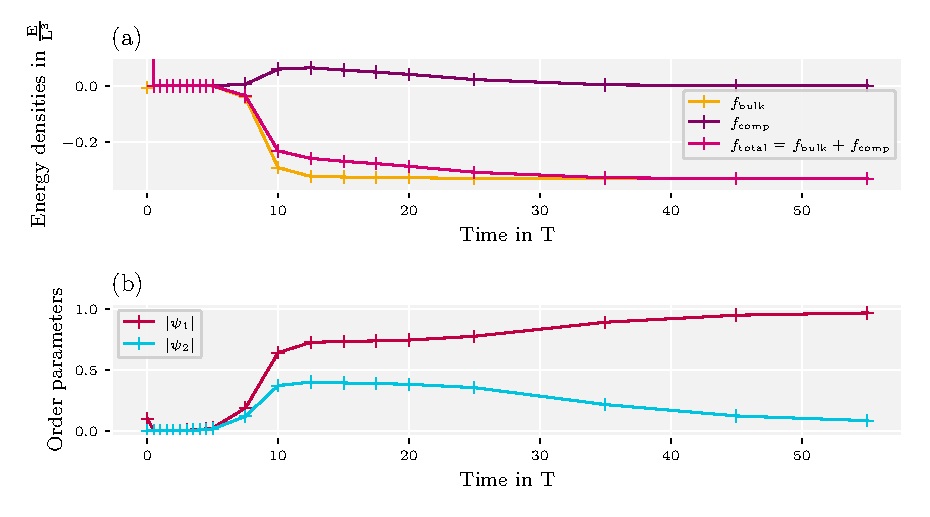
\includegraphics{figures/data_plots/fiso_r7_energies.pdf}
            \end{center}
            \caption{
                Dynamics of the free energy and order parameters in time of the large quench-like simulation described in \cref{sec:nr_quench}.
                (a) shows the volume averaged free energy densities \FB, \FC\ and their sum. \FU\ is not present as we have $K=b_2=0$.
                The values of the energy densities are cut off for the initial state which had $\FC\sim1\si{\frac{E}{L^3}}$.
                We see how at first the dynamics are driven by the deformation energy before $f_\text{total}$ starts following \FB\ with a noticeable bump of \FC\ when the system starts getting ordered again and so gradients grow.
                (b) shows the volume averaged order parameters of a biaxial \EE\ as given by \cref{eq:Ebiax}.
            }\label{fig:fiso_r7e}
        \end{figure}

        \begin{figure}[t!]
            \begin{center}
                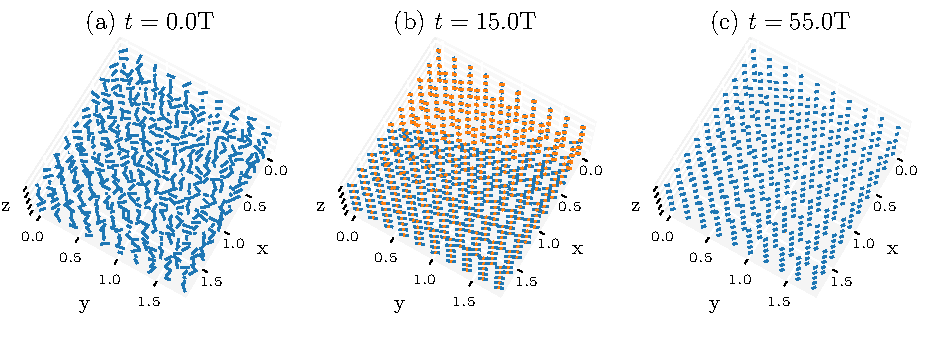
\includegraphics{figures/data_plots/fiso_r7_sample.pdf}
            \end{center}
            \caption{
                Snapshots showing the reconstructed layer normal directors \NN\ and \MM\ of an approximately $2\si{L}\times2\si{L}\times1\si{L}$ region of the large quench-like simulation discussed in \cref{sec:nr_quench} at selected times.
                The directors are shown as headless arrows to highlight their parity symmetry, which is present in our model.
                \NN\ which is always associated with the dominant order at a particular point is shown in blue whereas \MM\ is shown in orange.
                Here the director \NN\ is shown normalized with constant magnitude whereas \MM\ is scaled by the biaxial order parameter $|\psi_2|$ to highlight that (a) and (c) are uniaxial.
                In contrast, (b) shows a high degree of biaxiality with at least two domains being clearly visible in the region.
            }\label{fig:fiso_r7s}
        \end{figure}

        This simulation has been done on a cube box of 101 grid points for each dimension making for a total system size of $10.1\si{L}\times10.1\si{L}\times10.1\si{L}$, which is towards the upper end of what we can comfortably run, and was ran for a total time of $55\si{T}$.
        We specifically wanted to run a large system for this setup as during a quench from a random isotropic state, as the system starts getting ordered it is possible for multiple independent domains to develop and grow.
        Though this can of course only occur if the system is large enough for the initial domains to be sufficiently separated.
        As they continue growing they at some point meet, defects form and they either annihilate or we get a final static state with defects.
        Such an effect has been observed by Paget et al in 2D, however in 3D defect dynamics often radically change due to the additional degrees of freedom.
        In our quench simulations we never saw any defects appear.
    
        Coming back to the simulation we present here, the first thing we see is that the randomly generated initial state has a very high deformation energy costs due to its sharp gradients, see \cref{fig:fiso_r7e}.
        As such we first get a short period of further melting where $|\psi|$ reaches $10^{-3}$ and as that happens it presumably gets easier for the \NN\ and potentially also \MM\ to align.
        Then by the time the order starts growing again all the nearby directors are aligned, and we get relatively strong biaxiality with order present in two orthogonal directions throughout the volume and some slight long range deformation (not visible in the data we show).
        Importantly however, due to the biaxiality we see a smooth transition between what would otherwise look like two separate domains.
        This is as the split between the two orders is not uniform in volume, there are regions where one of them is distinguishably larger than the other and vice versa.
        This can be seen in \cref{fig:fiso_r7s}(b) where we show snapshots of the two directors \NN\ and \MM\ in different colors, however as we always associate \NN\ with the larger order (we have $|\psi_1| > |\psi_2|$ as discussed in \cref{sec:npE_wwbE}) we can clearly see two regions.

        From this we conclude that the system size and initial configuration was suitable for the development of separate domains but either due to the nature of 3D defects and their dynamics, or due to the present biaxiality of \EE\ which makes it easier to smoothly transition between domains we always end up at a uniform final state.
        Besides the simulation presented, we have also done multiple smaller scale simulations with $K=0$ and varying initializations, and one large scale simulation with $K=1$ all resulting in a uniform final state.
        It is worth noting however, that in the smaller scale simulations we do not always get a uniaxial (or nearly) final state.
        In fact for a series of smaller simulations of cube systems with side length of $3.1\si{L}$ and $K=0$ we consistently ended up with a final state of both $|\psi_2|$ and $|\psi_1|$ being approximately 0.5 and $|\psi_1|-|\psi_2|\sim0.1$.
        This suggests that biaxiality in 3D is a larger and more present problem than we initially hoped as it can occur even in relatively simple systems and it does not go away at large times.

    \subsection{Bridge-like states}\label{sec:nr_bs}
        \begin{figure}[t!]
            \begin{center}
                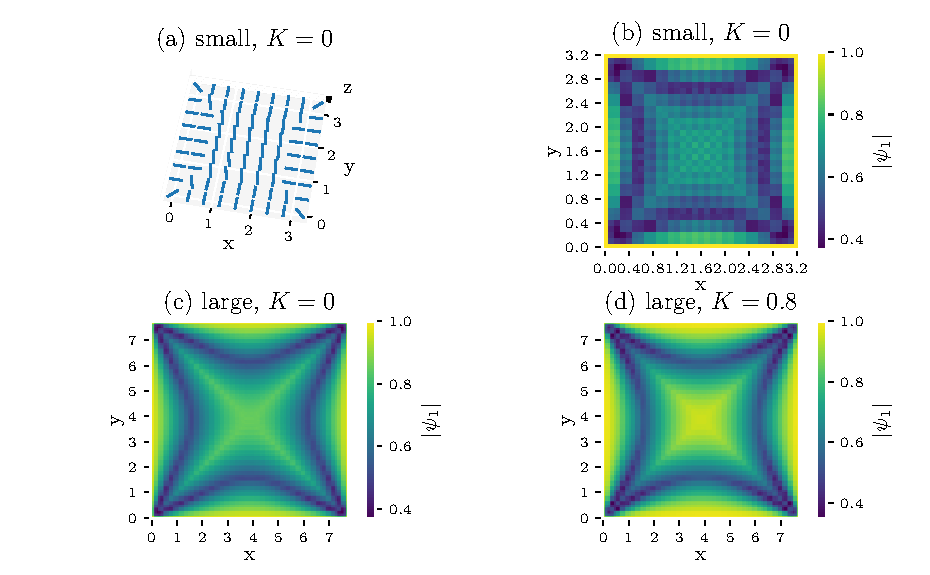
\includegraphics{figures/data_plots/fbox_r12_cross.pdf}
            \end{center}
            \caption{
                Escaping into the third dimension and the characteristic X shape of simulations with homeotropic boundaries along their sides only, as discussed in \cref{sec:nr_bs}.
                (a) and (b) show the layer normal direction \NN\ and the order parameter $|\psi_1|$ respectively for the final state of a relatively small simulation of side length $3.2\si{L}$ and $K=0$.
                (c) and (d) show only the smectic order parameter $|\psi_1|$ for a similar but larger simulation with them having the Ginzburg parameter $K$ be 0 and 0.8 respectively.
            }\label{fig:fbox_cross}
        \end{figure}
        We now move to simulations of a more complex system partially inspired by the observed strong presence of biaxiality in \EE\ and recent results by Monderkamp et al\cite{a.monderkampTopologicalFineStructure2022,monderkampTopologyOrientationalDefects2021}.
        Monderkamp et al have performed particle based simulations of confined rod-like molecules in 2D and 3D analysing their smectic structure.
        They suggest the use of a tetratic order parameter due to the presence of long defect lines (planes in 3D) with ends resembling point defects of $\pm\frac{1}{4}$ topological charge.
        These defect lines correspond to domain walls between two smectic structures with perpendicular direction of layering.
        Given the biaxiality present in \EE\ and how that seems to encourage boundaries where \NN\ switches to be perpendicular we thought that perhaps a biaxial 3D \EE\ might be well compatible with the use of said tetratic order parameter.

        Further, in the 3D simulations Monderkamp et al observe what they call bridge states\cite{a.monderkampTopologicalFineStructure2022}, these are composed of a couple of uninterrupted smectic layers span the system, which have the mentioned defect lines bordering a perpendicular layering on either side.
        Now, they simulate cylindrically shaped systems which our simulator is not well suited for, and in addition in their final state they mainly observe homogenous anchoring where the layers form perpendicular to the surface, which is also something that we cannot do well with our current fixed boundaries.
        So what we do is by no means a direct analogy, but regardless we attempted to find similar bridge-like final states using the fixed homeotropic boundaries described in \cref{sec:ns_sb}.

        First, we attempted to find these bridge states using boundaries only on the sides of our cuboid system while keeping the top and bottom $xy$-plane faces periodic.
        Such a setup always resulted with some order spreading from the boundaries, but what see mainly is \NN\ escaping into the third dimension and aligning with $\hat{\su{z}}$, see \cref{fig:fbox_cross}(a).
        This happens mainly in the middle and in the corners where the system is most frustrated with the order becoming particularly strong in the middle far away from the boundaries.
        The same behaviour has been observed for a large variety of systems ranging in system side length from 5 to $15\si{L}$ and with the Ginzburg parameter ranging from 0 to 1.2, the order parameter field for some of these is shown in \cref{fig:fbox_cross}(b-d), with a distinctive X pattern appearing.

        Besides changing the system side, we have also tried changing the anchoring near the corners as they seemed to have an outsized influence on the system.
        Without going into the details, we have smoothened the boundary \EE\ near the corners (${\sim}.3\si{L}$) by pointing \NN\ towards the centre of a sphere/cylinder placed in that corner.
        However, this had very little effect with all the data shown in \cref{fig:fbox_cross} using this method and still showing the same signs.
        We also use an adaptation of these rounded corners in the next system we discuss.

        Seeing that we do not see any bridge states for homeotropic boundaries from the sides only, but certainly see plenty of perpendicular \NN\ boundaries, the natural next step is to add boundaries along the last two faces of the system too.
        From a practical standpoint however, this means we have to simulate a full cube with large sizes in all three dimensions, whereas before we could only simulate a thin slab due to the system symmetry.
        This comes with a limitation on the system size that we can reasonably simulate.
        As such, we have done a systematic search of these bridge states with varying $K$ and with cube sided length ranging from 1.1 to $4.1\si{L}$, however these did not show anything interesting.
        They form a 3D adaptation of the X shape of \cref{fig:fbox_cross} while maintaining symmetry and having a low $|\EE|$ in the middle, see \cref{fig:3dfbox_longside}(c,d) for an example.

        \begin{figure}[t!]
            \begin{center}
                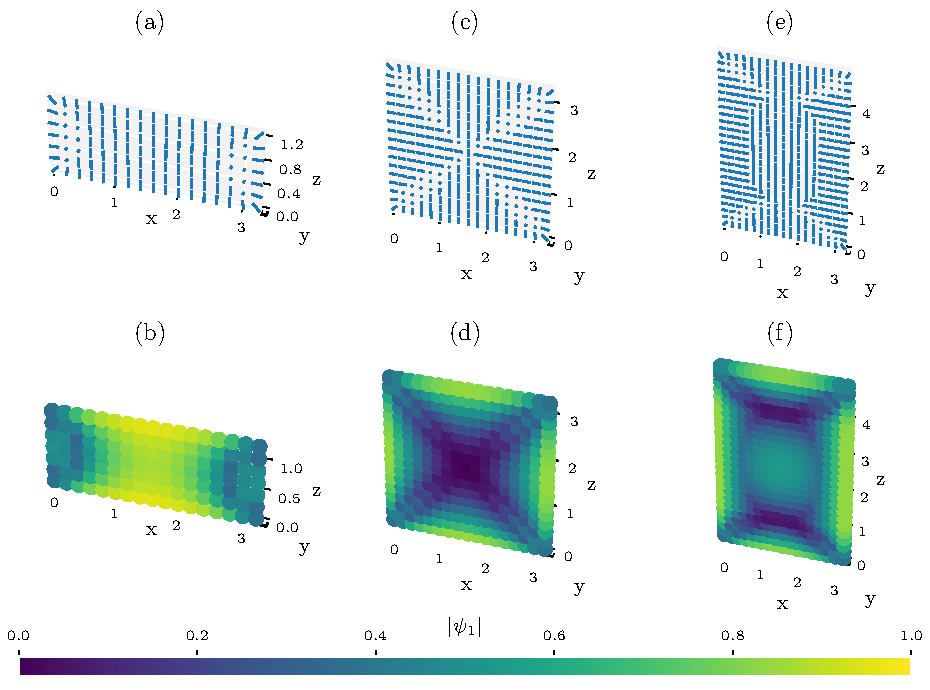
\includegraphics{figures/data_plots/3dfbox_r17_side.pdf}
            \end{center}
            \caption{
                Cross-sections of final states of simulations with homeotropic boundaries on all sides, $K=0$, size in the $x$ and $y$ directions of $3.6\si{L}$ and different heights.
                (a,c,e) show the layer normal direction \NN\ in blue, \MM\ is not shown as we have $|\psi_2| \ll |\psi_1|$.
                (b,d,f) show the order parameter field $|\psi_1|$.
                (a,b) are for a height of $1.6\si{L}$ where we clearly see a bridge-like state spanning the short dimension.
                (c,d) are for a height of $3.6\si{L}$ making the system fully symmetric, and we get a melted phase in the middle.
                (e,f) are for a height of $5.1\si{L}$ which contains another separated domain in the middle which escapes into the third dimension similarly to \cref{fig:fbox_cross}.
            }\label{fig:3dfbox_longside}
        \end{figure}

        \begin{figure}[t!]
            \begin{center}
                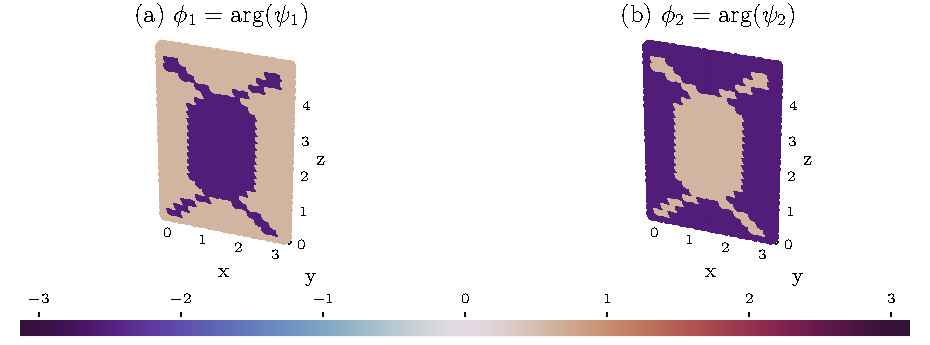
\includegraphics{figures/data_plots/3dfbox_r17_sidephi.pdf}
            \end{center}
            \caption{
                Cross sections of the phases $\phi_1, \phi_2$ of the complex order parameters $\psi_1, \psi_2$ in the final state of the simulation corresponding to \cref{fig:3dfbox_longside}(e,f).
                We have very sharp boundaries as a result of the \EE\ eigenvalue selection process of \cref{sec:npE_wwbE} and the two phases are always shifted exactly by $\pi$.
            }\label{fig:3dfbox_longsidephi}
        \end{figure}

        % Besides that we have done two more studies on these frustrated systems.
        % Firstly, we artificially break the cubic symmetry by keeping the system size the same for $x$ and $y$ but changing its height.
        Besides this, we have also performed simulations where we artificially break the cubic symmetry by keeping the system size the same for $x$ and $y$ but changing its height.
        For this we have run one series of simulations with $K=0$, still the one constant approximation free energy, the $x$ and $y$ size of the system being $3.6\si{L}$ and varying the height from 1.6 to 5.1\si{L}.
        These systems are very sensitive to whether the height is less than or greater than the system with of $3.6\si{L}$, cross-sections of final state \NN\ and $|\psi_1|$ for a selection of heights are shown in \cref{fig:3dfbox_longside}

        At small heights we perhaps unsurprisingly get a bridge-like state crossing the shorter height and we get a correspondingly large degree of ordering.
        As we cross the height of $3.6\si{L}$ where the system becomes symmetric we get a decrease in total ordering and finally as the height gets larger than the system width we get a completely different configuration.
        In this regime we get short ranged order near each boundary and then another bubble-shaped domain of order in the middle.
        This order has a layering normal direction \NN\ aligned to $\hat{\du{z}}$ just as the top and bottom phases, however despite this we get a clear boundary between the two where order decreases to $|\psi_1|\sim0.05$.
        This is very surprising and suggests there is likely something wrong with the model, this very likely being the allowed biaxiality of \EE\ and how it interplays with the complex phases of $\psi_1$ and $\psi_2$.

        We can see why the model shows a melting boundary between the two when we examine the phases $\phi_1$ and $\phi_2$ of $\psi_1$ and $\psi_2$, their cross-sections for the run with height $5.1\si{}$ are shown in \cref{fig:3dfbox_longsidephi}.
        There we immediately see two things, we have very sharp boundaries in both phase fields and that the two form perfectly matching domains that have values shifted by $\pi$.
        The sharp boundaries are not in themselves a major issue as they are an effect of the biaxial \EE\ deconstruction process detailed in \cref{sec:npE_wwbE} where we choose to always take $|\psi_1| > |\psi_2|$, it is thus really only a sign that the two orders have switched and \EE\ is still smooth.
        We can also explain the difference in the two phases always being $\pi$ using the theory from \cref{sec:npE_wwbE} where we have shown that precisely this would be energetically favourable as decreases \FB\ while not needing to change $|\psi_1|$ or $|\psi_2|$.
        It is also worth noting that we have observed this same behaviour for the complex phase fields in nearly all our simulations.
        As such we conclude that the earlier discussed biaxiality-enabled transition between two domains of order with a perpendicular \NN\ can only take place if the dominant orders in these domains have their complex phases differ by $\pi$.

        As such we suspect that the initial order in the bubble domain of \cref{fig:3dfbox_longside} was formed via an escape to the third dimension through biaxiality and as such has grown with a complex phase differing by $\pi$ to that of the boundaries (which we set to all have the same phase).
        This then later prevents this domain and that growing from the top and bottom boundaries to merge, as while they have the same \NN\ they have strongly differing complex phases neither of which can change.
        This means that while the biaxiality of \EE\ is still likely an issue and something that needs to be further studied, this particular problem could just as well be resolved by implementing more realistic boundary conditions which may allow the complex phase to change at the boundary and so for the domains to merge.

    \subsection{Imposed twist}\label{sec:nr_it}
        The main overarching theme of this thesis and in particular the simulation results is that biaxiality plays a much larger role than we initially expected and hoped.
        In particular, it allows for a smooth \EE\ field to still translate to sharp boundaries between domains of perpendicular \NN.
        As such, for our final set of simulations we focus on a simpler case that might allow us to better quantify how this transition comes to be.

        \begin{figure}[t!]
            \begin{center}
                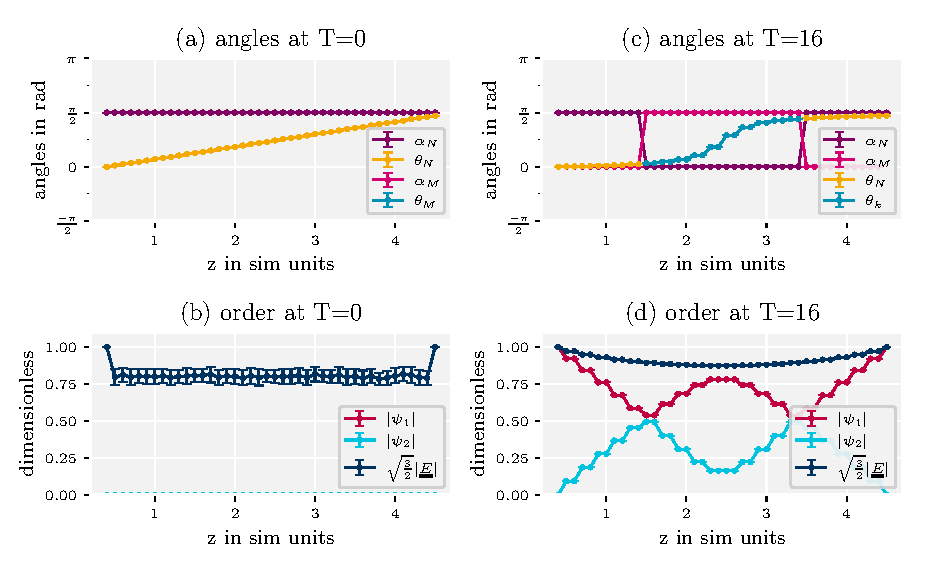
\includegraphics{figures/data_plots/twist_angleseg.pdf}
            \end{center}
            \caption{
                An example initial and final (at time $16\si{T}$) state configurations for an imposed twist of $\Delta\theta=0.47\pi$ and system height of 4.1\si{L}.
                All quantities are averaged over the $x$ and $y$ dimensions with standard deviations shown.
                (a, c) show the polar angles as defined in \cref{sec:nr_it} of the eigenvectors of \EE\ \NN\ and \MM.
                We only observe $\alpha$ angles of 0 or $\frac{\pi}{2}$ which correspond to the vector being aligned with $\hat{\su{z}}$ or laying in the $xy$ plane respectively.
                (b, d) Show the order parameters.
                In particular panels (c) and (d) are interesting where we can see a growing polar order which overtakes the $xy$ plane order in the middle section.
            }\label{fig:twist_angleseg}
        \end{figure}

        In these simulations we use PBCs for the $x$ and $y$ dimensions but have a fixed boundary for top and bottom faces.
        In these we as usual set $|\psi|=1$ and $\phi$ to an arbitrary constant and we set \NN\ to be aligned with $\hat{\su{x}}$ in the bottom face, but set it to a different direction within the $xy$ plane at the top face.
        Furthermore, we initialize \EE\ throughout the bulk to be uniaxial with a gradually twisting \NN\ so that it meets both boundaries, and a partially randomized $|\psi|$ an $\phi$.
        We denote the total angle by which the director rotates as $\Delta\theta$ and note that given the initialization this may be more than $\frac{\pi}{2}$.
        We have also ran similar simulations with a randomized \NN\ in the bulk, however the results were indistinguishable so we focus on this initialization.
        
        With these simulations we want to determine under which conditions does the system prefer a smooth deformation between the two boundaries and when does it escape into the third dimension as we have been seeing, in particular we expect the total twist $\Delta\theta$ and the system height $H$ to play a role.
        Given that we really study this as a one dimensional problem, we average all quantities over the $x$ an $y$ dimensions, in all our simulations the system quickly collapsed into being completely uniform along those.

        We employ spherical coordinates to be able to quantify the direction of \NN\ as a function of $z$.
        However, to avoid confusion with the complex phase $\phi$ we use the letter $\alpha$ to denote the spherical altitude angle and the letter $\theta$ for the azimuthal angle (this corresponds to our notation of $\Delta\theta$).
        See \cref{fig:twist_angleseg} for an example of what these quantities look like as a function of $z$.

        We ran multiple series of simulations varying $\Delta\theta$ from 0.06$\pi$ to 0.75$\pi$ and system height $H$ from 1.1 to 9.1\si{L}.
        Throughout these simulations we have seen significant biaxiality, with the exception of simulations with a very low $\Delta\theta$.
        We exclusively see two orderings, one we call inplane which is the one that we initialize the system with and has its layer normal direction in the $xy$ plane.
        The other we call the polar order which always has its layer normal direction aligned with $\hat{\su{z}}$ and which we again attribute to a biaxial escape into the third dimension.
        We also always see these two orders change continuously as a function of $z$ with perhaps the exception of $\Delta\theta = \frac{\pi}{2}$.
        As such, so that we do not have to account for the discontinuously changing \NN\ and \MM\ (see \cref{fig:twist_angleseg}(d)) which always represent the highest order as opposed to a particular type, we define the order parameters \sL\ and \sL\ along with their associated layer normal directions \aL\ and \aP.
        These correspond to the two observed types of orderings respectively.
        From now on we will only use \sL, \sP\ and the azimuthal angle of the \aL\ which we call simply $\theta$ as all the other angles are (near) constant.

        \begin{figure}[t!]
            \begin{center}
                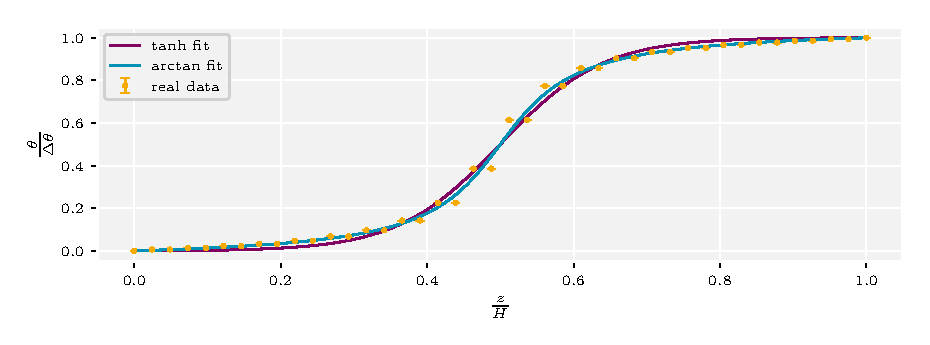
\includegraphics{figures/data_plots/twist_fits.pdf}
            \end{center}
            \caption{
                Comparison of the $\arctan$ and $\tanh$ fits to the non-dimensionalized function relation $\frac{\theta}{\Delta\theta}$ vs $\frac{z}{H}$ for the final state of the same simulation as is used for \cref{fig:twist_angleseg}.
            }\label{fig:twist_fits}
        \end{figure}

        \begin{figure}[t!]
            \begin{center}
                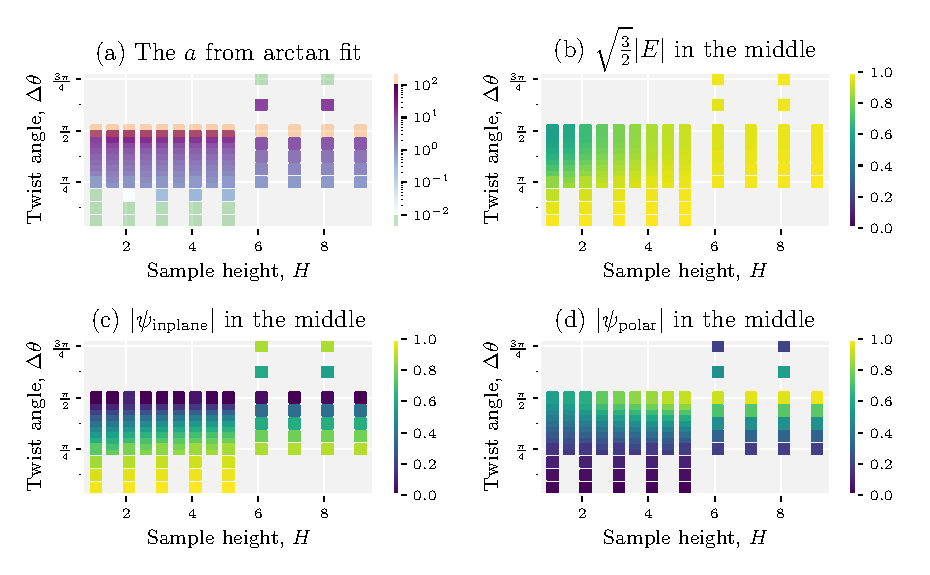
\includegraphics{figures/data_plots/twist_K0_outline.pdf}
            \end{center}
            \caption{
                Combined data from all our twist runs with $K=0$ usng the one constant approximation free energies, the $a$ parameter represents the sharpness of the rotation of the inplane order, larger $a$ means a very localized transition.
                (b,c,d) show the order parameters which are related via \cref{eq:bEcontr}, overall we unsurprisingly see the inplane order dominates at low twist angles.
                More interesting is that while the polar order is generally stronger at higher $\Delta\theta$, at low enough $H$ it also decreases suggesting the gradients can overpower it and a certain amount of space is needed for \EE\ to escape into the third dimension.
            }\label{fig:twist_K0_outline}
        \end{figure}

        We now want to quantify the shape of how the azimuthal angle $\theta$ changes as a function of $z$.
        To do that, we first of all non-dimensionalize these quantities and instead look at $\frac{\theta}{\Delta\theta}$ as a function of $\frac{z}{H}$.
        This way the shapes can be compared irrespective of these quantities.
        The form shown in \cref{fig:twist_angleseg} clearly looks sigmoidal (as do others) and so we attempted to fit the data using both $\arctan$ and $\tanh$ functions, which once suitably adjusted so that they pass through the points $(0, 0), (\frac{1}{2}, \frac{1}{2})$ and $(1, 1)$ in the $\frac{\theta}{\Delta\theta}$ vs $\frac{z}{H}$ plane each have one remaining free parameter.
        Both fits performed well for the smoother more linear transitions, however the $\arctan$ matched the shape of the $\frac{\theta}{\Delta\theta}$ vs $\frac{z}{H}$ relation much better, see \cref{fig:twist_fits} for a comparison, as such from now on we only use the $\arctan$ fits which are given by
        \begin{equation}\label{eq:fit}
            \frac{\theta}{\Delta\theta} = \frac{\arctan(a \qty(\frac{z}{H} - \frac{1}{2}))}{2\arctan(\frac{a}{2})} + \frac{1}{2}
        \end{equation}
        with $a$ being the remaining dimensionless parameter.
        For an intuition, the resulting sigmoid is very line-like for $a < {\sim}0.5$ and becomes very sharp at $a\sim100$, we also have the slope of this function in the middle given by
        \begin{equation}
            \eval{\dv{\frac{\theta}{\Delta\theta}}{\frac{z}{H}}}_\text{middle} = \frac{a}{2\arctan(\frac{a}{2})}
        \end{equation}
        which directly corresponds to how sharp the transition is.

        We then summarize all our simulations results for $K=0$ in \cref{fig:twist_K0_outline}.
        There we see the mentioned parameter $a$ along with the three order parameters $\sqrt{\frac{3}{2}}|\EE|$, $|\psi_1|$ and $|\psi_2|$, which all have values in the range 0 to 1, as measured at the centre of the sample at height $\frac{H}{2}$ with the $x$ and $y$ dimensions again being averaged over.
        Interestingly, while we have originally expected the simulation results to collapse and be only a function of the parameter $\frac{\Delta\theta}{H}$ we were unable to find such a relation.
        The only clear information we are able to extract from $a$ is that the transition remains smooth and continuous at all angles except at $\Delta\theta =\frac{\pi}{2}$.
        We have repeated these simulations for $K$ of 0.4 and 1 as well but they are qualitatively very similar, the only difference being that with higher $K$ results behave as if their system height was smaller in comparison.

        \begin{figure}[t!]
            \begin{center}
                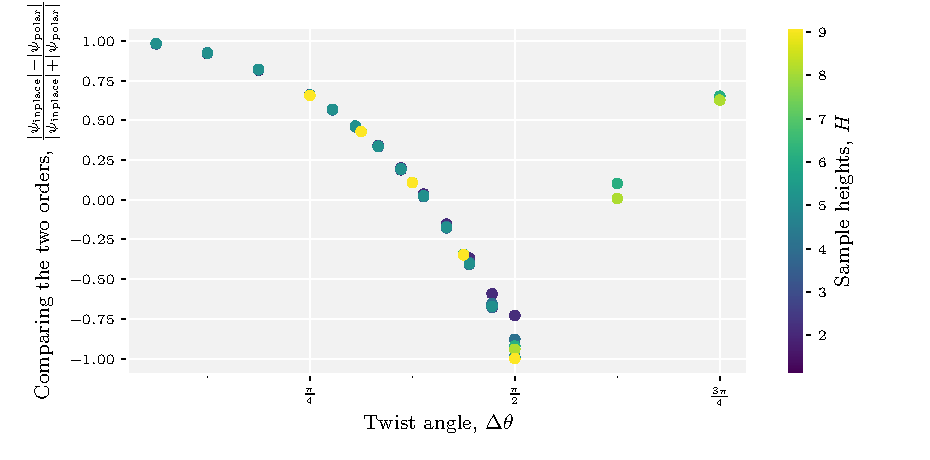
\includegraphics{figures/data_plots/twist_K0_coll.pdf}
            \end{center}
            \caption{
                The data from \cref{fig:twist_K0_outline} collapses onto a single curve (nearly) irrespective of sample height $H$ when we only look at which of the two orders dominates in the middle region.
            }\label{fig:twist_K0_coll}
        \end{figure}

        However, we did find that when only comparing whether the inplane or the polar order dominates in the centre via middle of the system quantities from \cref{fig:twist_K0_outline} as we do in \cref{fig:twist_K0_coll}, the data shows nearly no dependence on system height.
        This once again suggests that the biaxiality we have present in \EE\ acts like a superposition of two nearly independent layering orders, unless they are forced to interact like in the last part of \cref{sec:nr_bs}
        It is also worth pointing out how for $\Delta\theta > \frac{\pi}{2}$, where we initialize the director \NN\ as overtwisted, we see the same final states as for those related by $\Delta\theta \rightarrow \pi - \Delta\theta$.
        In these systems we first see a raise of polar order as the inplane order diminishes and then regrows with the direction of \NN\ now twisting in the other direction where the total twist is smaller.
        Thus, the overtwisted systems in effect melt and then reorder as systems of total twist $\pi - \Delta\theta$ but in the other direction, this agrees with the data in \cref{fig:twist_K0_coll}.
        This suggests these final states are very stable and further shows how easily the biaxial \EE\ overcomes any energy barriers.

        \begin{figure}[t!]
            \begin{center}
                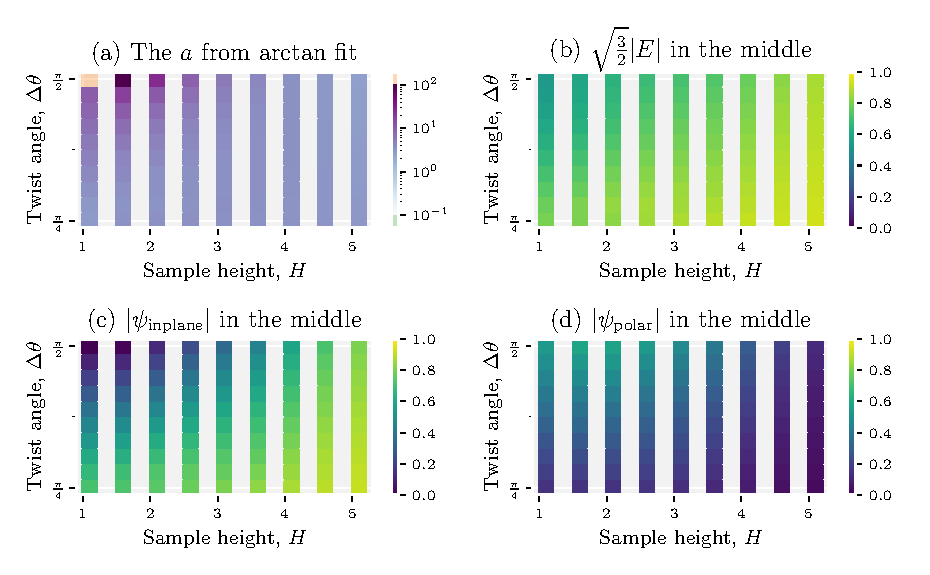
\includegraphics{figures/data_plots/twist_outline_POs.pdf}
            \end{center}
            \caption{
                An equivalent plot to \cref{fig:twist_K0_outline} but for simuations using the intuitive smectic free energy form and $K=0$.
                Here we see that $a$ is much less likely to become very high even at $\Delta\theta = \frac{\pi}{2}$ and $|\psi_\text{polar}|$ is very low and decreases with $H$.
            }\label{fig:twist_outline_POs}
        \end{figure}

        Finally, we have also run a smaller selection of these simulations with the intuitive smectic free energy form where we have $b_1^\perp=b_2^\parallel=b_2^{\parallel\perp}=0$.
        For these we currently only have data for $\Delta\theta \leq \frac{\pi}{2}$ and $K=0$.
        The final states were found to have the same functional forms with respect to height $z$ as those of \cref{fig:twist_angleseg} and so we still fit the shape of the twist angle to height relation using \cref{eq:fit} as before and show the data in \cref{fig:twist_outline_POs}.
        This looks markedly different, we no longer always have a near step function transition in the twist angle for the inplane order when $\Delta\theta = \frac{\pi}{2}$.
        This sharp transition now only develops at the smallest system heights and beyond it we start getting a very smooth, linear transition of $a\sim1$ even at $\Delta\theta=\frac{\pi}{2}$.
        This means that unlike the in one constant approximation free energy version, the initial conitions matter, as if initialized with a melted middle the system would be symmetric and not be able to choose in which directon to develop the twist.

        In addition, we get a much smaller $|\sP|$ compared to the one constant approximation free energy and it has the opposite behaviour when it comes to system height $H$ changing.
        While before the polar order grew at larger heights somewhat suggesting that with the one constant approximation free energy the system preferred to escape into the third dimension under a twist but could only do so well if it had sufficient space for it.
        We now only ever get the polar order at the most perpendicular $\Delta\theta$ and the smallest system heights, suggesting it only forms as a last resort due to extreme frustration of the system.
        This shows that choosing the right form of the free energy (including our projection operator free energy) can also help mitigate the observed biaxiality in our systems.
        And perhaps that the intuitive smectic free energy we use here does show configurations more similar to real smectic systems than the one constant approximation.


\section{Conclusion}
    \EE\ theory is one of multiple theoretical frameworks currently being developed for a better understanding of smectic liquid crystals.
    It continues in the spirit of the de Gennes complex order parameter and brings new inspirations from the nematic \QQ\ tensor to better incorporate the fundamental symmetry of smectics.
    It is one of few mesoscopic order parameters being actively developed to solve the symmetry problem highlighted by Pevnyi et al.
    As such, while it is still early in its development, due to its mesoscopic nature and numerical convenience \EE\ theory might be a very good candidate for large scale numerical simulations including defects.

    In this thesis we provide a comprehensive overview of the de Gennes inspired order parameters, the issues they face and how \EE\ attempts to solve it.
    In \cref{sec:Ei} we provide a fully comprehensive introduction to \EE\ theory including how it relates to the physical density wave and explain all details of its dynamics.
    We then tackle the first goal of this project, extending \EE\ theory to 3D.
    This was more complex than initially expected and lead to a full review of what exactly \EE\ should be in \cref{sec:npE}.
    There we have proven that constraining the complex tensor \EE\ to be symmetric, traceless and normal fully implies it will take the biaxial form of \EE\ in 3D and the uniaxial form in 2D.
    We have concluded that constraining \EE\ to be uniaxial in 3D would require constraining its eigenvalues and concluded that to be analytically impossible and numerically too expensive, and as such we have for the time being accepted a biaxial \EE.
    Finalizing the extension to 3D, we review how we can use Lagrange multipliers to enforce the constraints on \EE.
    We then present a clear and concise way to express our constraints as real-valued holonomic constraints and show how we can use soft constraints for our Lagrange multipliers.

    We then move to what was the second major goal of this project, to finalize the projection operator free energy form suggested by Paget et al and to compute the corresponding functional derivatives.
    We then also address the previously overlooked problem of taking the complex square root when approximating \PP\ and we managed to find a procedure to fully correct any branch cut problems.
    Finally, we implement a numerical solver which iteratively solves the \EE\ dynamics partial differential equation in 3D including all the new theoretical additions.

    Finally, we run three sets of simulations, starting with a simple quench-like system where we do not observe any defect formation and always arrive at a uniform final state.
    We attempt to simulate more complex frustrated systems where we impose different \EE\ from different boundaries and we observe a strong effect of the layer normal \NN\ escaping into the third dimension.
    Finally, we try to find at what angle dod we have to impose nearby layer normal directors \NN\ for the system become too biaxial and escape into the third dimension.
    There we find that an anlge of ${\sim}\frac{3\pi}{8}$ is sufficient for the perpendicular order to become dominant.

\newpage
\printbibliography[heading=bibintoc]

\newpage
\begin{appendices}
    \section{Equivalency of $[\EE,\EE^*]=0$ and $\det([\EE,\EE^*])=0$ in 2D}\label{app:noruaeq}
        Consider \EE\ to be a 2D, symmetric, traceless and otherwise unrestricted complex matrix given by
        \begin{equation}
            \EE = \begin{pmatrix}
                a & b \\
                b & -a \\
            \end{pmatrix}
        \end{equation}
        with $a, b \in \mathbb{C}$.
        The commutator $[\EE,\EE^*]$ will be given by
        \begin{equation}
            [\EE,\EE^*] = \du{K} - \du{K}^* \qq{with} \du{K} = \begin{pmatrix}
                a & b \\
                b & -a \\
            \end{pmatrix} \cdot \begin{pmatrix}
                a^* & b^* \\
                b^* & -a^* \\
            \end{pmatrix} = \begin{pmatrix}
                |a|^2 + |b|^2 & ab^* - a^*b \\
                ba^* - ab^* & |a|^2 + |b|^2 \\
            \end{pmatrix}
        \end{equation}
        so that
        \begin{equation}
            [\EE,\EE^*] = \begin{pmatrix}
                0 & d - d^* \\
                d^* - d & 0 \\
            \end{pmatrix} = (d-d^*) \begin{pmatrix}
                0 & 1 \\
                -1 & 0 \\
            \end{pmatrix}
        \end{equation}
        where
        \begin{equation}
            d = ab^* - a^*b \qq{and} d^* = a^*b - ab^* = -d
        \end{equation}
        so we finally arrive at
        \begin{align}
            [\EE,\EE^*] &= 2 (ab^* - a^*b) \begin{pmatrix}
                0 & 1 \\
                -1 & 0 \\
            \end{pmatrix} \\
            \det([\EE,\EE^*]) &= 2 (ab^* - a^*b)
        \end{align}
        So clearly requiring either of the two is equivalent to requiring $ab^*-a^*b = 0$ and so they are equivalent to each other.
    \section{The smectic symmetries}
        This section was originally intended for a dedicated discussion section of the report which was later removed as it was clear there was not enough space or time to write it in.
        Nevertheless we include it here as it may of interest to anyone further thinking about \EE.

        Earlier, in the motivational part of this thesis we have mentioned that one of the advantages of \EE\ is that it respects the symmetry of reversing the layering direction \NN\ both globally and locally.
        While this is the true symmetry of a layered system, it is not a symmetry of the established relation between $|\psi|,\phi,\su{N}$ and the density modulation
        \begin{equation}\label{eq:lim_den2}
            \rho(\su{r}) = \rho_0 + \Re(|\psi| e^{i(q_0\ssu{N}\cdot\ssu{r} + \phi)}), \qq{$|\psi|,\su{N}$ and $\phi$ being fields}
        \end{equation}
        which we did not directly use in this work, but it heavily guided our interpretation of the field.
        The only symmetry of \cref{eq:lim_den2} is under simultaneously exchanging $\su{N}, \phi \leftrightarrow -\su{N}, -\phi$ locally or globally.
        There are naturally two ways to resolve this issue.
        Either modify \EE, in particular its complex phase, such that it respects the symmetry of \cref{eq:lim_den2}.
        Or find a different way to interpret the fields from \EE\ as it is, or perhaps a combination of both approaches.

        For modifying \EE, we suspect this would be very difficult to the point where any suitable form of \EE\ would likely be so different it should be called something else.
        This is as one would need to somehow couple the complex phase $\phi$ and \NN, an eigenvector of \EE, which is only accessible numerically.
        This is as the only symmetry of \cref{eq:lim_den2} is when the signs of both flip, not just one.
        Regardless, if one was to find a form for \EE\ that satisfied both symmetries independently the interpretation of $\phi$ would not hold anymore.
        Currently, using \cref{eq:lim_den2}, we interpret $\dv{\phi}{x}$ (with $x$ being the direction along \NN\ at any point) as a contraction if it is positive and dilation if negative.
        However, the change of $\phi \rightarrow -\phi$ will change the sign of these and so clearly this is not a physical symmetry of the system.

        Thus, it seems the more natural way to move forward is to adapt \cref{eq:lim_den2} to respect the symmetry in \NN\ only.
        Starting from a wave resembling $e^{i(\ssu{q_0}\cdot\ssu{r})}$ of which we want to adjust the wavelength locally.
        Given the addition in \cref{eq:lim_den2} using $e^{i(\ssu{q_0}\cdot\ssu{r})(1+s(\ssu{r}))}$ might be a good starting point, where $s=0$ corresponds to equilibrium spacing, $s>1$ to a contraction and $s<1$ to a dilation.
        This form has the required symmetry and can be expanded as
        \begin{equation}
            e^{i(\ssu{q_0}\cdot\ssu{r})(1+s(\ssu{r}))} = e^{i(q_0\ssu{N}\cdot\ssu{r} + s(\ssu{r})q_0\ssu{N}\cdot\ssu{r})} 
        \end{equation}
        which now has the same form as \cref{eq:lim_den2} with $\phi(\su{r}) = s(\su{r})q_0\su{N}\cdot\su{r}$, however it is very important to stress that that would no longer be the $\phi$ from \EE\ as that would not change anything.
        However, $s$ and $\phi$ from \EE\ are both dimensionless quantities and perhaps we can find a way to map them onto each other.
        The only reasonable values for $s$ are from $-1$, where the wavelength becomes infinite, to $+\inf$ where wavelength goes to 0.
        Any values $<-1$ would just correspond to a different $s$ and a flipped $\su{N}$.
        On the other hand $\phi$ from \EE\ belongs to any set interval of length $2\pi$.
        So if we use $\phi \in (-\pi, \pi]$ and let $s = \frac{\phi}{\pi}$ then the model could account for any dilation and a contraction of up to half the natural wavelength.
        However, this would fundamentally change what $\phi$ from \EE\ is and would require more work to investigate the free energy costs to contractions and dilations, among other considerations.

\end{appendices}


\end{document}
